%%%%%%%%%%%%%%%%%%%%%%%%%%%%%%%%%%%%%%%%
% Compact Laboratory Book
% LaTeX Template
% Version 1.0 (4/6/12)
%
% This template has been downloaded from:
% http://www.LaTeXTemplates.com
%
% Original author:
% Joan Queralt Gil (http://phobos.xtec.cat/jqueralt) using the labbook class by
% Frank Kuster (http://www.ctan.org/tex-archive/macros/latex/contrib/labbook/)
%
% License:
% CC BY-NC-SA 3.0 (http://creativecommons.org/licenses/by-nc-sa/3.0/)
%
% Important note:
% This template requires the labbook.cls file to be in the same directory as the
% .tex file. The labbook.cls file provides the necessary structure to create the
% lab book.
%
% The \lipsum[#] commands throughout this template generate dummy text
% to fill the template out. These commands should all be removed when 
% writing lab book content.
%
% HOW TO USE THIS TEMPLATE 
% Each day in the lab consists of three main things:
%
% 1. LABDAY: The first thing to put is the \labday{} command with a date in 
% curly brackets, this will make a new section showing that you are working
% on a new day.
%
% 2. EXPERIMENT/SUBEXPERIMENT: Next you need to specify what 
% experiment(s) and subexperiment(s) you are working on with a 
% \experiment{} and \subexperiment{} commands with the experiment 
% shorthand in the curly brackets. The experiment shorthand is defined in the 
% 'DEFINITION OF EXPERIMENTS' section below, this means you can 
% say \experiment{pcr} and the actual text written to the PDF will be what 
% you set the 'pcr' experiment to be. If the experiment is a one off, you can 
% just write it in the bracket without creating a shorthand. Note: if you don't 
% want to have an experiment, just leave this out and it won't be printed.
%
% 3. CONTENT: Following the experiment is the content, i.e. what progress 
% you made on the experiment that day.
%
%%%%%%%%%%%%%%%%%%%%%%%%%%%%%%%%%%%%%%%%%

%----------------------------------------------------------------------------------------
%    PACKAGES AND OTHER DOCUMENT CONFIGURATIONS
%----------------------------------------------------------------------------------------                               

% \UseRawInputEncoding

\documentclass[fontsize=11pt, % Document font size
                             paper=letter, % Document paper type
                             %twoside, % Shifts odd pages to the left for easier reading when printed, can be changed to oneside
                             openany, % chapters can start on any page
                             captions=tableheading,
                             index=totoc,
                             hyperref]{labbook}

%\documentclass[idxtotoc,hyperref,openany]{labbook} % 'openany' here removes the
  
\usepackage[bottom=10em]{geometry} % Reduces the whitespace at the bottom of the page so more text can fit

\usepackage[english]{babel} % English language
\usepackage{lipsum} % Used for inserting dummy 'Lorem ipsum' text into the template

\usepackage[utf8]{inputenc} % Uses the utf8 input encoding
\usepackage[T1]{fontenc} % Use 8-bit encoding that has 256 glyphs

\usepackage[osf]{mathpazo} % Palatino as the main font
\linespread{1.05}\selectfont % Palatino needs some extra spacing, here 5% extra
\usepackage[scaled=.88]{beramono} % Bera-Monospace
\usepackage[scaled=.86]{berasans} % Bera Sans-Serif

\usepackage{booktabs,array} % Packages for tables

\usepackage{amsmath} % For typesetting math
\usepackage{graphicx} % Required for including images
\usepackage{etoolbox}
\usepackage[norule]{footmisc} % Removes the horizontal rule from footnotes
\usepackage{lastpage} % Counts the number of pages of the document
\usepackage{float}




\usepackage[dvipsnames]{xcolor}  % Allows the definition of hex colors
\usepackage{epstopdf}
\epstopdfsetup{suffix={}}
\definecolor{titleblue}{rgb}{0.16,0.24,0.64} % Custom color for the title on the title page
\definecolor{linkcolor}{rgb}{0,0,0.42} % Custom color for links - dark blue at the moment

\addtokomafont{title}{\Huge\color{titleblue}} % Titles in custom blue color
\addtokomafont{chapter}{\color{OliveGreen}} % Lab dates in olive green
\addtokomafont{section}{\color{Sepia}} % Sections in sepia
\addtokomafont{pagehead}{\normalfont\sffamily\color{gray}} % Header text in gray and sans serif
\addtokomafont{caption}{\footnotesize\itshape} % Small italic font size for captions
\addtokomafont{captionlabel}{\upshape\bfseries} % Bold for caption labels
\addtokomafont{descriptionlabel}{\rmfamily}
\setcapwidth[c]{10cm} % Center align caption text
\setkomafont{footnote}{\sffamily} % Footnotes in sans serif

\deffootnote[4cm]{4cm}{1em}{\textsuperscript{\thefootnotemark}} % Indent footnotes to line up with text

\DeclareFixedFont{\textcap}{T1}{phv}{bx}{n}{1.5cm} % Font for main title: Helvetica 1.5 cm
\DeclareFixedFont{\textaut}{T1}{phv}{bx}{n}{0.8cm} % Font for author name: Helvetica 0.8 cm

\usepackage{scrhack}
\usepackage[headsepline]{scrlayer-scrpage} % Provides headers and footers configuration
\pagestyle{scrheadings} % Print the headers and footers on all pages
\clearscrheadfoot % Clean old definitions if they exist

\automark[chapter]{chapter}
\ohead{\headmark} % Prints outer header

\setlength{\headheight}{25pt} % Makes the header take up a bit of extra space for aesthetics
\addtokomafont{headsepline}{\color{lightgray}} % Colors the rule under the header light gray

\ofoot[\normalfont\normalcolor{\thepage\ |\  \pageref{LastPage}}]{\normalfont\normalcolor{\thepage\ |\  \pageref{LastPage}}} % Creates an outer footer of: "current page | total pages"

% These lines make it so each new lab day directly follows the previous one i.e. does not start on a new page - comment them out to separate lab days on new pages
\makeatletter
\patchcmd{\addchap}{\if@openright\cleardoublepage\else\clearpage\fi}{\par}{}{}
\makeatother
\renewcommand*{\chapterpagestyle}{scrheadings}

% These lines make it so every figure and equation in the document is numbered consecutively rather than restarting at 1 for each lab day - comment them out to remove this behavior
\usepackage{chngcntr}
\counterwithout{figure}{labday}
\counterwithout{equation}{labday}

% Hyperlink configuration
\usepackage[
    pdfauthor={Kalli Allen, Darrah Beebe, and Jason Braker}, % Your name for the author field in the PDF
    pdftitle={Laboratory Journal}, % PDF title
    pdfsubject={labNotebookSeniorProject3}, % PDF subject
    bookmarksopen=true,
    linktocpage=true,
    urlcolor=linkcolor, % Color of URLs
    citecolor=linkcolor, % Color of citations
    linkcolor=linkcolor, % Color of links to other pages/figures
    backref=page,
    pdfpagelabels=true,
    plainpages=false,
    colorlinks=true, % Turn off all coloring by changing this to false
    bookmarks=true,
    pdfview=FitB]{hyperref}

\usepackage[stretch=10]{microtype} % Slightly tweak font spacing for aesthetics

\usepackage[framed,numbered,autolinebreaks,useliterate]{mcode}
\usepackage{todonotes}

% This package is for plotting graphs
\usepackage{pgfplots}

%\setlength\parindent{0pt} % Uncomment to remove all indentation from paragraphs

%----------------------------------------------------------------------------------------
%    DEFINITION OF EXPERIMENTS
%----------------------------------------------------------------------------------------

% Template: \newexperiment{<abbrev>}[<short form>]{<long form>}
% <abbrev> is the reference to use later in the .tex file in \experiment{}, the <short form> is only used in the table of contents and running title - it is optional, <long form> is what is printed in the lab book itself

\newexperiment{example}[Example experiment]{This is an example experiment}
\newexperiment{example2}[Example experiment 2]{This is another example experiment}
\newexperiment{example3}[Example experiment 3]{This is yet another example experiment}

\newsubexperiment{subexp_example}[Example sub-experiment]{This is an example sub-experiment}
\newsubexperiment{subexp_example2}[Example sub-experiment 2]{This is another example sub-experiment}
\newsubexperiment{subexp_example3}[Example sub-experiment 3]{This is yet another example sub-experiment}

%----------------------------------------------------------------------------------------
\newcommand{\HRule}{\rule{\linewidth}{0.5mm}} % Command to make the lines in the title page

\setlength\parindent{0pt} % Removes all indentation from paragraphs

\begin{document}

%----------------------------------------------------------------------------------------
%    TITLE PAGE
%----------------------------------------------------------------------------------------
%\frontmatter % Use Roman numerals for page numbers

%\begin{center}

%

\title{
\begin{center}
\href{http://www.bradley.edu}{
\includegraphics[height=0.5in]{figs/logoBU1-Print}}
\vskip10pt
\HRule \\[0.4cm]
{\Huge \bfseries Laboratory Notebook \\[0.5cm] \Large Robotic Cart}\\[0.4cm] % Degree
\HRule \\[1.5cm]
\end{center}
}
\author{ Kallistah Allen, Darrah Beebe, and Jason Braker \\ \\\Large kjallen@mail.bradley.edu, dbeebe@mail.bradley.edu, \\jbraker@mail.bradley.edu} % Your name and email address
\date{Beginning September 14, 2020} % Beginning date
\maketitle

%\maketitle % Title page

\printindex
\tableofcontents % Table of contents
\newpage % Start lab look on a new page

\begin{addmargin}[0cm]{0cm} % Makes the text width much shorter for a compact look

\pagestyle{scrheadings} % Begin using headers

%----------------------------------------------------------------------------------------
%    LAB BOOK CONTENTS
%----------------------------------------------------------------------------------------

\labday{Monday, September 14, 2020}
\experiment{Meeting Minutes}
JB\\
In today's meeting, Dr. Miah, Dr. Shastry, Kalli, and I set up a weekly meeting time on Mondays from 5:00 to 6:00 pm. Darrah was not present. Dr. Miah went over introductory materials and shared a Google Drive as well as a GitHub repo for storing files. We were informed by Dr. Miah that we should use camel case for file names. Dr. Miah also informed us that we will be using Inkscape or IPE for creating figures, and Dia for flowcharts. 

%-------------------------------------------

\labday{Monday, September 21, 2020}
\experiment{Meeting Minutes}
JB\\
In today's meeting, Dr. Miah gave us an overview of the LaTex files we will be using for our documentation. He briefly showed us how to edit and compile the LaTex documents. We were informed that the draft of our ECE 497 document containing block diagrams, requirements, and specifications is due on October 6, 2020. Also, the final version is due October 22, 2020.

%-------------------------------------------

\labday{Thursday, September 24, 2020}
\experiment{Meeting Minutes}
JB\\
Today Kalli, Darrah, and I met to come up with the inputs and outputs of the robotic cart system. We brainstormed together to come up with a list of inputs and outputs for both the robotic cart and the remote. We then assigned Kalli to draw the block diagram, Darrah to write a functional description of the blocks, and Jason to write the end-use requirements.

%-------------------------------------------

\labday{Tuesday, September 29, 2020}
\experiment{Meeting Minutes}
Agenda: Go over inputs/outputs of the system, as well as the end-use requirements and block descriptions.

\vspace*{12pt}

JB\\
The weekly meeting time was changed to 2:30 - 3:30 pm on Tuesdays.\\
In today's meeting, we presented the inputs and outputs that we came up with to Dr. Miah. Some of our inputs and outputs were too technical or low-level, so we simplified them to the inputs and outputs that the end user would see. Dr. Miah informed us that Dia is for flowcharts, not block diagrams, and that we should just use Inkscape for all of the figures, flowcharts, and block diagrams. We were reminded that we need to set up a 3 hour slot on Tuesdays and Thursdays for lab time and send Dr. Miah a Zoom link so he can attend.

%-------------------------------------------

\labday{Tuesday, October 6, 2020}
\experiment{CoppeliaSim Modeling}

JB\\
Today in the lab time, I worked on modeling the Junior Runt Rover robot in CoppeliaSim. First, I drew a 3d model of the robot chassis and a wheel in an external 3d CAD program. Then I imported the models into CoppeliaSim and worked on setting up the joints for simulation. I found the following document that explained how to model a robot in CoppeliaSim: \href{https://www.coppeliarobotics.com/helpFiles/en/buildingAModelTutorial.htm}{https://www.coppeliarobotics.com/helpFiles/en/buildingAModelTutorial.htm}

\vspace*{12pt}

KA\\
Today during the lab time, I worked on modeling the Junior Runt Rover robot in CoppeliaSim. First, I researched how to model a robot using the CoppeliaSim software and used the following document as a guide:\\
\href{https://www.coppeliarobotics.com/helpFiles/en/bubbleRobTutorial.htm}{https://www.coppeliarobotics.com/helpFiles/en/bubbleRobTutorial.htm}\\
Then I modeled the robot chassis based on preliminary measurements of the Junior Runt Rover and then opened a new scene to design each of the wheels and worked on configuring the wheels to the chassis of the robot.

\vspace*{12pt}DB\\
For this lab session I found and used the same reference material as linked by Jason.  I then measured and modded the Actobotics Junior Rover in Fusion 360 and imported it into Coppelia Sim and finished linked the model together.  Did not get to but next step should be getting it connected to Matlab.

\experiment{Meeting Minutes}
Agenda:
\begin{itemize}
    \item Discuss next steps in project
    \item Discuss Xbee modules and project materials
\end{itemize}

JB\\
In today's meeting, we briefly went over the System Level Functional Requirements document with Dr. Shastry since he missed our meeting last week. Then we were informed that we need to make a presentation from the material in that document. The presentation will be next Tuesday, October 13th, in our weekly meeting. Finally, we discussed the Xbee modules. Darrah already has enough Xbee modules, and Kalli and I will go to Dr. Miah's office to pick up some modules to use for the project.

%-------------------------------------------

\labday{Thursday, October 8, 2020}
\experiment{System Level Presentation}

JB\\
Today we worked on the presentation of the system level functional requirements for ECE 497. We created a presentation containing the information from our system level document. This presentation will be given on Tuesday, October 13, 2020. We decided that Kalli will present the introduction, Darrah will present the system architecture, and Jason will present the specifications.

\experiment{CoppeliaSim Modeling}
JB\\
After working on the presentation, I worked on my CoppeliaSim model of the Runt Rover. I was able to get my model running and successfully completing the point navigation lab from ECE 444.

\vspace*{12pt}DB\\
Between now and the last lab meeting I got the model connected to Matlab but not functioning fully accurately yet.  Spent the remainder of the time after the System level diagram was put together cleaning up the Coppelia model to be more friendly to use and align some axis that were aligned incorrectly.

\vspace*{12pt}
KA\\
After we finished the presentation slides I worked on the CoppeliaSim model of the Junior Runt Rover. I was able to apply the front and rear wheel axles to the robot model. Once the cart was fully assembled I ran a simple test code on it to make sure all the parts were applied correctly and that the robot would move.

%-------------------------------------------

\labday{Tuesday, October 13, 2020}
\experiment{Lab Session}
DB\\
Lab was canceled today to work on Dr. Miah's test instead during the time.

%-------------------------------------------

\labday{Thursday, October 15, 2020}
\experiment{CoppeliaSim Model}
JB\\
Today we worked on the CoppeliaSim model. We found that if we commanded the robot with $v = 0$ [m/s] and $\omega = \pi/2$ [rad/s] for 1 second, the robot did not turn $\pi/2$ radians as expected. After looking at the math for a while, we determined that we needed to modify our definition of the distance between the wheels. Previously, we were using the distance between the left wheels and the right wheels, but the actual circle that the wheels follow when turning will have a diameter equivalent to the diagonal distance between wheels (for example, the distance from the front left wheel to the rear right wheel). Also, the linear speed of the wheels is not tangent to the circular path the wheels must follow. Therefore, we need to only account for the tangential component. The final formula we got for the left and right wheel speeds ($v_L$ and $v_R$ respectively) were
$$v_L = v - \frac{\omega L^2}{2d_{LR}}$$
$$v_R = v + \frac{\omega L^2}{2d_{LR}}$$
where $d_{LR}$ is the distance between the left and right wheels.

\vspace*{12pt}DB\\
The Following math is what we worked out during lab and uses the variables from \autoref{fig:rotMathDiagram}. The first step is to define the Actual velocity for rotation, $v_A$, and map it to wheel velocity, $v$, where $\theta_A$ is the angle between the ideal tangent velocity to the rotation and the wheels velocity.  Then use new axle length, $L$, along with actual velocity to get new rotational velocity equation from wheel velocities.

\begin{center}
\renewcommand{\arraystretch}{1.5}
\begin{tabular}{ c | c | c }
    \begin{math}
        \begin{array}{c}
        $$\theta_{A} = atan(L_{2}/L_{1})$$\\
        $$L = \sqrt{(L_{1})^2+(L_{2})^2}$$
        \end{array}
    \end{math} &
    \begin{math}
        \begin{array}{c}
        $$v = v_{A}*cos(\theta_{A})$$\\
        $$cos(\theta_{A}) = L_{1}/L$$\\
        $$v = v_{A}*\frac{L_{1}}{L}$$
        \end{array}
    \end{math} &
    \begin{math}
        $$\begin{array}{rcl}
        w &=& \frac{v_{AR}-v_{AL}}{L}\\
          &=& \frac{\frac{L_1}{L}(v_R-v_L)}{L}\\
          &=& \frac{L_1}{L^2}(v_R-v_L)
        \end{array}$$
    \end{math} \\
\end{tabular}
\end{center}
The resulting equations for mapping the rovers wheels to a unicycle are now put together.  The linear velocity equation is not modified since linear velocity is still perpendicular with the rovers wheel alignments.  For the angular velocity equation the coefficient on its main $(w_R-w_L)$ term of wheel speed difference has been modified to reflect the modified turning radius and the wheels offset orientation from the path they rotate on.

$$v = \frac{r}{2}(w_R+w_L)$$
\vspace*{-12pt}
$$w = \frac{rL_1}{L^2}(w_R-w_L)$$
\vspace*{12pt}

Next substitution in used to get the left and right angular wheel speeds, $w_R$ and $w_L$.

\vspace*{-18pt}
\begin{center}
\renewcommand{\arraystretch}{1.5}
\begin{tabular}{ c | c | c }
    \begin{math}
        $$\begin{array}{rcl}
        v &=& \frac{r}{2}(w_R+w_L)\\
        w_R &=& \frac{2v}{r}-w_L
        \end{array}$$
    \end{math} &
    \begin{math}
        $$\begin{array}{rcl}
        w &=& \frac{rL_1}{L^2}(w_R-w_L)\\
        w &=& \frac{rL_1}{L^2}((\frac{2v}{r}-w_L)-w_L)\\
        w_L &=& (v - \frac{w}{2}\frac{L^2}{L_1})/r
        \end{array}$$
    \end{math} &
    \begin{math}
        $$\begin{array}{rcl}
        w_R &=& \frac{2v}{r}-((v - \frac{w}{2}\frac{L^2}{L_1})/r)\\
        w_R &=& (v + \frac{w}{2}\frac{L^2}{L_1})/r\\
        \end{array}$$
    \end{math} \\
\end{tabular}
\end{center}
\vspace*{12pt}

Now we have the final angular wheel velocity equations in terms of robot velocity, $v$, robot angular velocity, $w$, axle length, $L_1$, wheel radius, $r$, and turning diameter, $L$.
\vspace*{-6pt}
$$\alpha = \frac{L^2}{2L_1}$$
\vspace*{-12pt}
$$w_R = \frac{v + {\alpha}w}{r}$$
$$w_L = \frac{v - {\alpha}w}{r}$$

\begin{figure}
    \center
    \includegraphics[width=5.5in]{figs/roatationalVelocityMathDiagram}
    \caption{Diagram for Rotational Velocity mapping}
    \label{fig:rotMathDiagram}
\end{figure}

\vspace*{12pt}
KA\\
During the lab time I was able to execute a point navigation code on my CoppeliaSim robot model. During the first run I had some inaccuracies in the robot's movement but the robot was able to navigate to the point [1.5, 1.5]. I also observed that my simulation time was too large since the robot would spin in circles, once it reached the target point, until the simulation time was finished. I plan to fix these movement errors and timing issues in the next lab day by using the equations Jason and Darrah came up with in the lab today.
%-------------------------------------------

\labday{Tuesday, October 20, 2020}
\experiment{XBee Training}

JB\\
In today's lab session, Darrah went over what he knows about the XBee modules and the code he has written for interfacing with them. He also informed us that from his experimentation, it may be very difficult to get a good distance measurement from signal strength when there are obstacles present. After that, I worked on creating the appendix to explain how to model the Runt Rover in CoppeliaSim.

\vspace*{12pt}
KA\\
In the lab session our group discussed the XBee modules and Darrah shared the code he wrote for communicating with the XBee modules. After going through Darrah's code I worked on assembling the motor connections for the Junior Runt Rover but ran into issues while stripping the wires for the BeagleBone Blue motor connection. 

\experiment{Meeting Minutes}
Agenda:
\begin{itemize}
    \item Give System Level Functional Requirements Presentation
    \item Discuss XBee external circuitry
\end{itemize}

JB\\
In today's meeting, we gave our presentation to Dr. Miah and Dr. Shastry. Their main point of feedback was that for future presentations, we should use more figures and videos to help convey what we are talking about. We were also encouraged to research existing solutions to following robots. We were also encouraged to research the multipath phenomenon, which causes signal strength variations due to the environment (walls, ceiling, floor, objects in the room, etc.).

%-------------------------------------------

\labday{Thursday, October 22, 2020}
\experiment{Linear Speed Testing}

KA\\
In today's lab session I compiled a list of parts to start the excel spreadsheet. As a group we came up with some parts and I researched the best website to order the parts from. After I had the initial sites of where to order from I saved the information to a word document so that we could get approval from Dr. Miah on what parts we needed before I entered them into the excel document. After I had the word document completed I then worked on putting together a c code for the junior runt rover in order to run the motors and test duty cycles.

\vspace*{12pt}
JB\\
Today, I worked on experimentally finding the relationship between duty cycle applied to the wheels and linear speed. To do this, I applied the same duty cycle to all wheels to run the Runt Rover alongside a measuring tape. I then measured the time it took for the Runt Rover to move 4 feet along the tape. From this, I calculated the linear speed. I repeated this 3 times for each duty cycle and averaged the results. The results of these experiments are shown in Tables \ref{tab:duty0.1} - \ref{tab:duty1.0}.

\begin{table}[h!]
    \centering
    \begin{tabular}{r|r|r|r}
        \toprule
        \textbf{Distance [ft]} & \textbf{Time [s]} & \textbf{Linear Speed [ft/s]} & \textbf{Linear Speed [m/s]}\\
        \toprule
        4.0 & 21.10 & 0.1896 & 0.05779\\
        4.0 & 20.99 & 0.1906 & 0.05810\\
        4.0 & 21.43 & 0.1867 & 0.05691\\
        \bottomrule
        \multicolumn{3}{r|}{\textbf{Average Linear Speed [m/s]}} & 0.05760\\
        \bottomrule
    \end{tabular}
    \caption{Experimental data with duty cycle 0.1}
    \label{tab:duty0.1}
\end{table}

\begin{table}[h!]
    \centering
    \begin{tabular}{r|r|r|r}
        \toprule
        \textbf{Distance [ft]} & \textbf{Time [s]} & \textbf{Linear Speed [ft/s]} & \textbf{Linear Speed [m/s]}\\
        \toprule
        4.0 & 7.47 & 0.5355 & 0.1632\\
        4.0 & 7.43 & 0.5384 & 0.1641\\
        4.0 & 7.47 & 0.5355 & 0.1632\\
        \bottomrule
        \multicolumn{3}{r|}{\textbf{Average Linear Speed [m/s]}} & 0.1635\\
        \bottomrule
    \end{tabular}
    \caption{Experimental data with duty cycle 0.2}
    \label{tab:duty0.2}
\end{table}

\begin{table}[h!]
    \centering
    \begin{tabular}{r|r|r|r}
        \toprule
        \textbf{Distance [ft]} & \textbf{Time [s]} & \textbf{Linear Speed [ft/s]} & \textbf{Linear Speed [m/s]}\\
        \toprule
        4.0 & 4.63 & 0.8639 & 0.2633\\
        4.0 & 4.60 & 0.8696 & 0.2651\\
        4.0 & 4.63 & 0.8639 & 0.2633\\
        \bottomrule
        \multicolumn{3}{r|}{\textbf{Average Linear Speed [m/s]}} & 0.2639\\
        \bottomrule
    \end{tabular}
    \caption{Experimental data with duty cycle 0.3}
    \label{tab:duty0.3}
\end{table}

\begin{table}[h!]
    \centering
    \begin{tabular}{r|r|r|r}
        \toprule
        \textbf{Distance [ft]} & \textbf{Time [s]} & \textbf{Linear Speed [ft/s]} & \textbf{Linear Speed [m/s]}\\
        \toprule
        4.0 & 3.40 & 1.176 & 0.3584\\
        4.0 & 3.37 & 1.187 & 0.3618\\
        4.0 & 3.33 & 1.201 & 0.3661\\
        \bottomrule
        \multicolumn{3}{r|}{\textbf{Average Linear Speed [m/s]}} & 0.3621\\
        \bottomrule
    \end{tabular}
    \caption{Experimental data with duty cycle 0.4}
    \label{tab:duty0.4}
\end{table}

\begin{table}[h!]
    \centering
    \begin{tabular}{r|r|r|r}
        \toprule
        \textbf{Distance [ft]} & \textbf{Time [s]} & \textbf{Linear Speed [ft/s]} & \textbf{Linear Speed [m/s]}\\
        \toprule
        4.0 & 2.68 & 1.493 & 0.4551\\
        4.0 & 2.64 & 1.515 & 0.4618\\
        4.0 & 2.65 & 1.509 & 0.4599\\
        \bottomrule
        \multicolumn{3}{r|}{\textbf{Average Linear Speed [m/s]}} & 0.4589\\
        \bottomrule
    \end{tabular}
    \caption{Experimental data with duty cycle 0.5}
    \label{tab:duty0.5}
\end{table}

\begin{table}[h!]
    \centering
    \begin{tabular}{r|r|r|r}
        \toprule
        \textbf{Distance [ft]} & \textbf{Time [s]} & \textbf{Linear Speed [ft/s]} & \textbf{Linear Speed [m/s]}\\
        \toprule
        4.0 & 2.25 & 1.778 & 0.5419\\
        4.0 & 2.27 & 1.762 & 0.5371\\
        4.0 & 2.24 & 1.786 & 0.5444\\
        \bottomrule
        \multicolumn{3}{r|}{\textbf{Average Linear Speed [m/s]}} & 0.5411\\
        \bottomrule
    \end{tabular}
    \caption{Experimental data with duty cycle 0.6}
    \label{tab:duty0.6}
\end{table}

\begin{table}[h!]
    \centering
    \begin{tabular}{r|r|r|r}
        \toprule
        \textbf{Distance [ft]} & \textbf{Time [s]} & \textbf{Linear Speed [ft/s]} & \textbf{Linear Speed [m/s]}\\
        \toprule
        4.0 & 1.88 & 2.128 & 0.6486\\
        4.0 & 1.87 & 2.139 & 0.6520\\
        4.0 & 1.89 & 2.116 & 0.6450\\
        \bottomrule
        \multicolumn{3}{r|}{\textbf{Average Linear Speed [m/s]}} & 0.6485\\
        \bottomrule
    \end{tabular}
    \caption{Experimental data with duty cycle 0.7}
    \label{tab:duty0.7}
\end{table}

\begin{table}[h!]
    \centering
    \begin{tabular}{r|r|r|r}
        \toprule
        \textbf{Distance [ft]} & \textbf{Time [s]} & \textbf{Linear Speed [ft/s]} & \textbf{Linear Speed [m/s]}\\
        \toprule
        4.0 & 1.71 & 2.339 & 0.7129\\
        4.0 & 1.65 & 2.424 & 0.7388\\
        4.0 & 1.64 & 2.439 & 0.7434\\
        \bottomrule
        \multicolumn{3}{r|}{\textbf{Average Linear Speed [m/s]}} & 0.7317\\
        \bottomrule
    \end{tabular}
    \caption{Experimental data with duty cycle 0.8}
    \label{tab:duty0.8}
\end{table}

\begin{table}[h!]
    \centering
    \begin{tabular}{r|r|r|r}
        \toprule
        \textbf{Distance [ft]} & \textbf{Time [s]} & \textbf{Linear Speed [ft/s]} & \textbf{Linear Speed [m/s]}\\
        \toprule
        4.0 & 1.48 & 2.703 & 0.8239\\
        4.0 & 1.47 & 2.721 & 0.8294\\
        4.0 & 1.45 & 2.759 & 0.8409\\
        \bottomrule
        \multicolumn{3}{r|}{\textbf{Average Linear Speed [m/s]}} & 0.8314\\
        \bottomrule
    \end{tabular}
    \caption{Experimental data with duty cycle 0.9}
    \label{tab:duty0.9}
\end{table}

\begin{table}[h!]
    \centering
    \begin{tabular}{r|r|r|r}
        \toprule
        \textbf{Distance [ft]} & \textbf{Time [s]} & \textbf{Linear Speed [ft/s]} & \textbf{Linear Speed [m/s]}\\
        \toprule
        4.0 & 1.30 & 3.077 & 0.9379\\
        4.0 & 1.29 & 3.101 & 0.9452\\
        4.0 & 1.30 & 3.077 & 0.9379\\
        \bottomrule
        \multicolumn{3}{r|}{\textbf{Average Linear Speed [m/s]}} & 0.9403\\
        \bottomrule
    \end{tabular}
    \caption{Experimental data with duty cycle 1.0}
    \label{tab:duty1.0}
\end{table}

The combined data for all of the tested duty cycles is in \autoref{tab:dutySpeed}. A duty cycle of 0 results in no movement of the robot, so the linear speed is 0.

\begin{table}[h!]
    \centering
    \begin{tabular}{c|c}
        \toprule
        \textbf{Duty Cycle} & \textbf{Linear Speed [m/s]}\\
        \toprule
        0.0 & 0\\
        0.1 & 0.0576\\
        0.2 & 0.1635\\
        0.3 & 0.2639\\
        0.4 & 0.3621\\
        0.5 & 0.4589\\
        0.6 & 0.5411\\
        0.7 & 0.6485\\
        0.8 & 0.7317\\
        0.9 & 0.8314\\
        1.0 & 0.9403\\
        \bottomrule
    \end{tabular}
    \caption{Measured speeds at various duty cycles}
    \label{tab:dutySpeed}
\end{table}

Using a 4th degree polynomial fit with the $y$-intercept fixed at 0, we can approximate this data with the following formula, where $v$ is the linear speed, and $d$ is the duty cycle applied:
\begin{equation}
    \label{eq:v(d)}
    v(d) = 1.2176d^4 - 2.5174d^3 + 1.6943d^2 + 0.5475d
\end{equation}
The scatterplot of the data with the curve of best fit is shown in \autoref{fig:v(d)bestfit}.

\begin{figure}[h!]
    \center
    \begin{tikzpicture}
        \begin{axis}[
            title={Linear Speed vs. Duty Cycle},
            xlabel={Duty Cycle},
            ylabel={Linear Speed [m/s]},
            xmin=0, xmax=1,
            ymin=0, ymax=1,
            xtick={0,0.1,...,1},
            ytick={0,0.1,...,1},
            legend pos=north west,
            xmajorgrids=true,
            ymajorgrids=true,
            width=4in,
        ]
            \addplot[
                color=blue,
                mark=o,
                mark size=2pt,
                only marks,
            ]
            table
            {
                x y
                0 0
                0.1 0.0576
                0.2 0.1635
                0.3 0.2639
                0.4 0.3621
                0.5 0.4589
                0.6 0.5411
                0.7 0.6485
                0.8 0.7317
                0.9 0.8314
                1.0 0.9403
            };
            \addlegendentry{Experimental Data}

            \addplot[
                domain=0:1,
                samples=100,
                color=blue,
            ]
            {1.2176*x^4 - 2.5174*x^3 + 1.6943*x^2 + 0.5475*x};
            \addlegendentry{4th Degree Polynomial of Best Fit}
        \end{axis}
    \end{tikzpicture}
    \caption{Best fit curve for speed and duty cycle}
    \label{fig:v(d)bestfit}
\end{figure}

%-------------------------------------------

\labday{Tuesday, October 27, 2020}
\experiment{Lab Time}

JB\\
Today we worked on putting together a list of parts since we cannot do much experimentation until we have the necessary parts. Dr. Miah advised us to get some external encoders as well as new motors with built-in encoders to allow us to detect wheel revolutions. We searched for motors with encoders, but it seems that we will have to do significant modification to the Runt Rover chassis to use most of the motors that are available. We decided to discuss this with Dr. Miah in our meeting this afternoon.

\vspace*{12pt}
KA\\
In today's lab I looked for a few research papers on the multipath issue Dr. Miah and Dr. Shastry informed us about on 10/20/2020 after our presentation. I made sure to add these research papers to the Google drive under the bibliography folder for use in our project. I also added a research paper about how to create a parabolic radio transceiver and what parts we would need in order to replicate this model. From last weeks lab I recorded the parts we needed for the project into the excel file for our project meeting today.

\experiment{Meeting Minutes}
Agenda: Discuss parts:
\begin{itemize}
    \item Encoders
    \item Motors
    \begin{itemize}
        \item Wheel motors
        \item Sensor motor - servo or stepper
    \end{itemize}
    \item Second Runt Rover kit
    \item Parabolic reflector
\end{itemize}

JB\\
In today's meeting, we discussed the possibility of buying external encoders to put on the wheels of the Runt Rover. We also discussed buying new motors with built-in encoders. Most of the motors that are available would require significant modification to the Runt Rover chassis. There was one motor (\href{https://www.amazon.com/Motor-Encoder-motor-120-integrated/dp/B07412V7WQ/ref=sr_1_8?dchild=1&keywords=TT+encoder+motor&qid=1603810303&sr=8-8#descriptionAndDetails}{TT Motor with Encoder}) that looks as though it would be able to be mounted in the same way as the existing motors. However, the maximum speed of this motor is $160 RPM$, which only yields a linear speed of approximately $0.5 m/s$. We determined that for this project, we may not be able to acheive the $2 m/s$ speed that we initially specified. Since this is a proof-of-concept, we decided that we want a speed of $1 m/s$. After discussing the motors some more, Dr. Miah showed us a different robot chassis that he has in his office. It is a chassis with two drive wheels and a caster, as shown in \autoref{fig:diffDriveChassis}. This chassis seems to be a better option for our project, so Dr. Miah is going to look for more of them. Since we are likely to switch to this chassis, we decided to hold off on getting encoders, motors, or Runt Rover kits for now.

\begin{figure}[h!]
    \center
    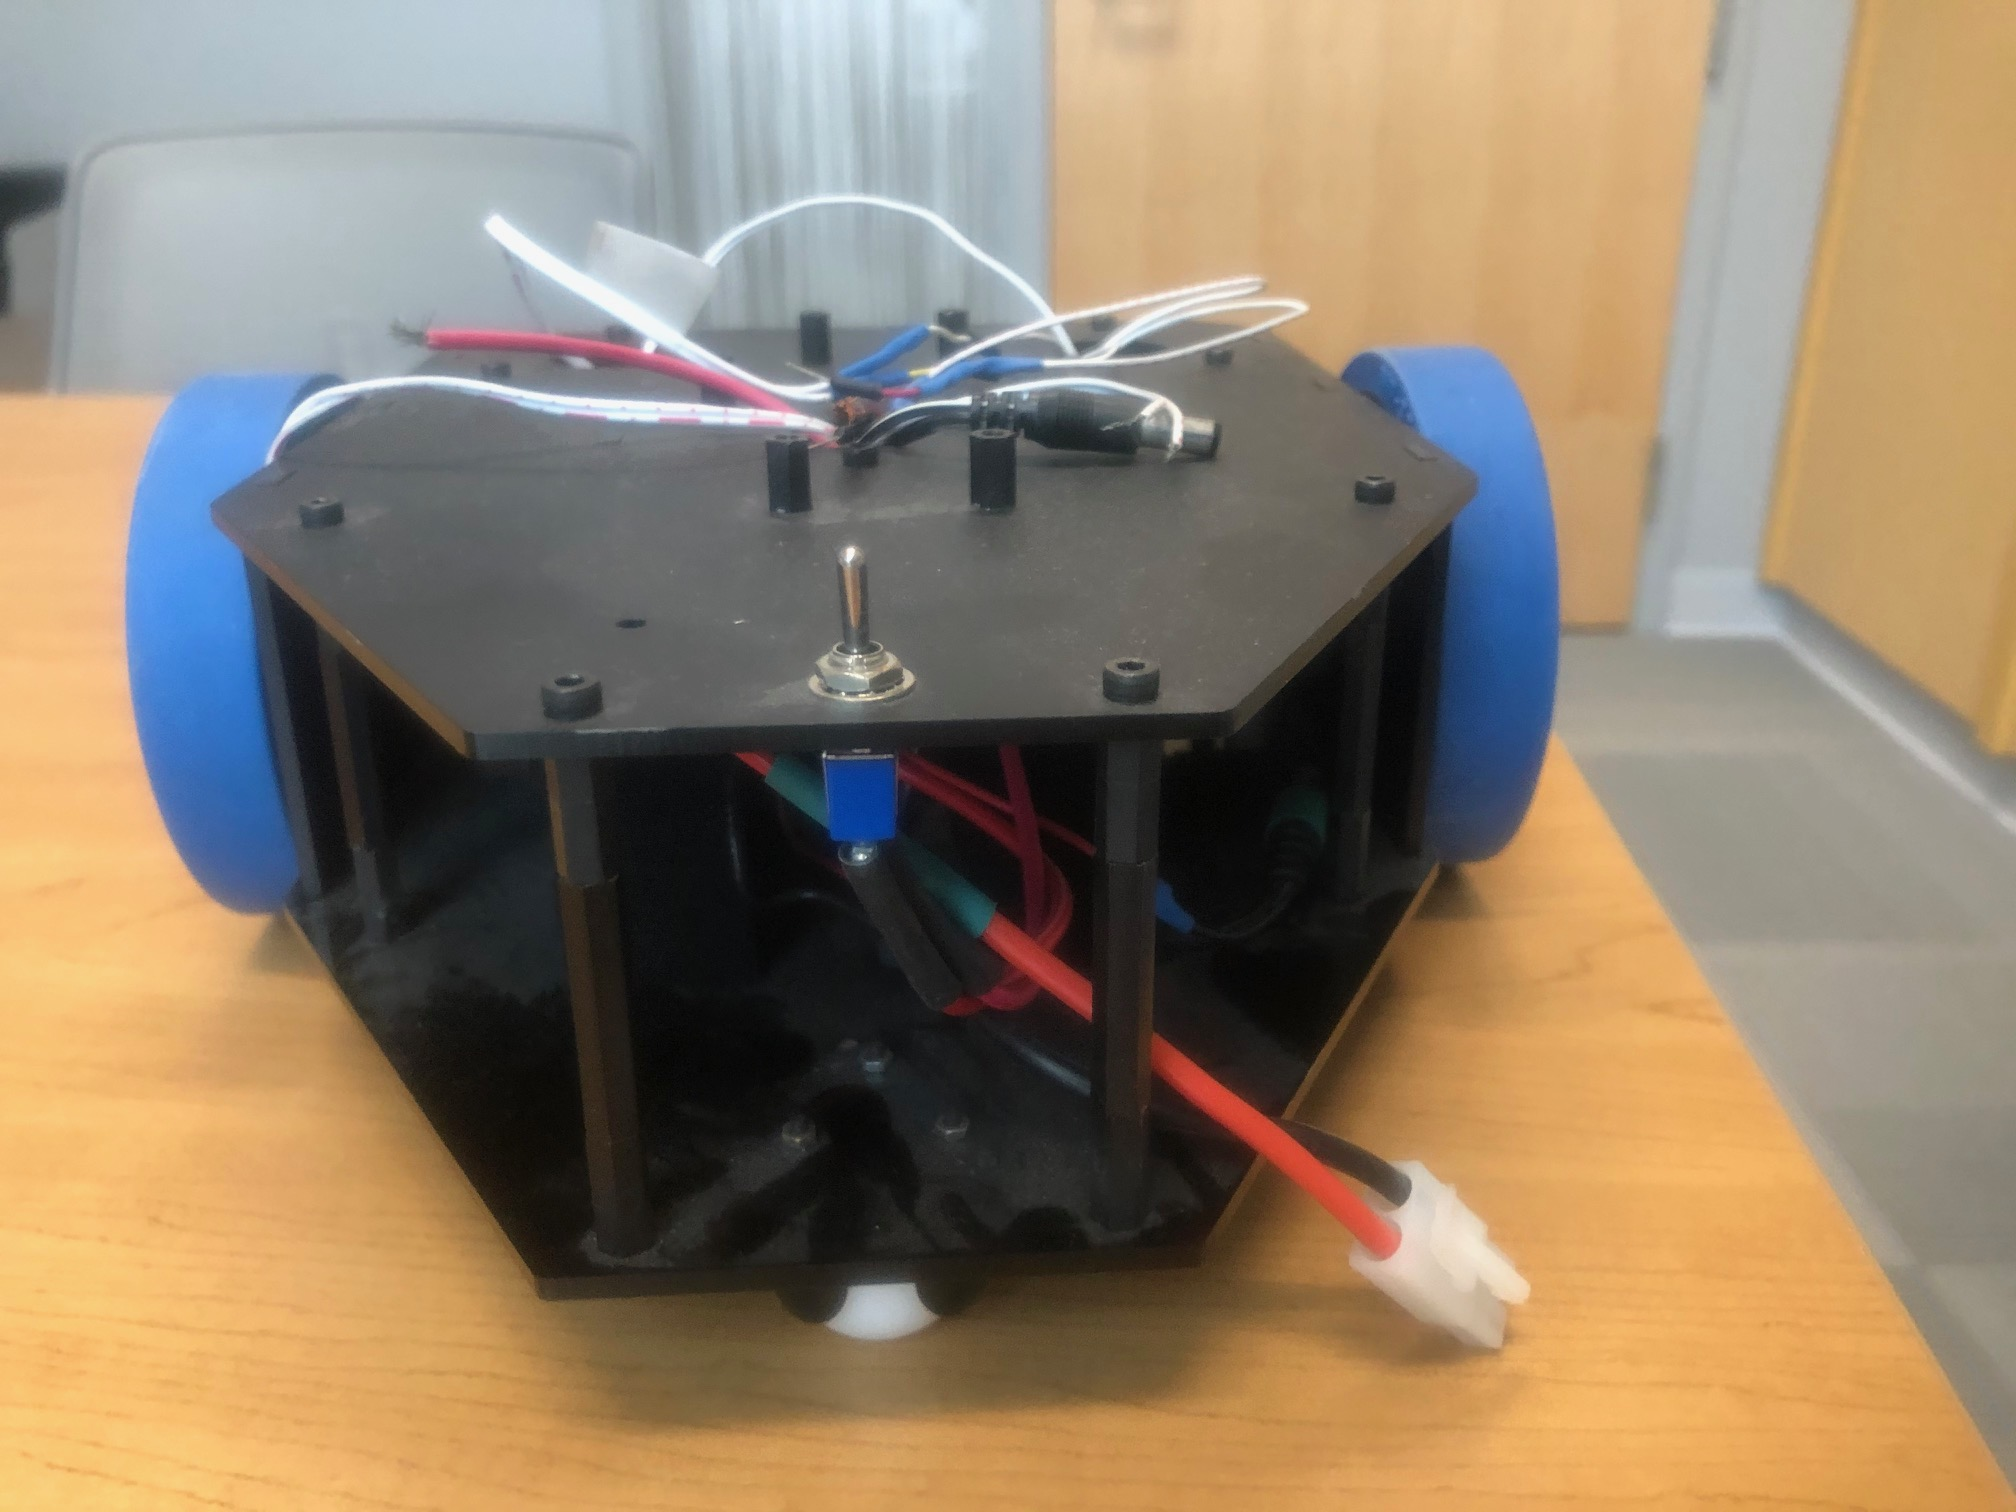
\includegraphics[width=4.5in]{figs/img/diffDriveChassis}
    \caption{Proposed Robot Chassis}
    \label{fig:diffDriveChassis}
\end{figure}

Finally, we discussed the parabolic reflector to directionalize the XBee sensor that will be mounted on the robot. Dr. Miah gave us the link to a previous senior project (\href{http://ee.bradley.edu/projects/proj2017/ekf_slam/Downloads/downloads.html}{found here}) that used such a parabolic reflector and directed us to the lab notebook for more information. We plan to look at the information there and decide whether to use the same design or to modify it.

%-------------------------------------------

\labday{Thursday, October 29, 2020}
\experiment{Budget Bot Evaluation}

JB\\
Today, we researched the Budget Bot chassis to see if it would be a better option than the Runt Rover. The motors included in the Budget Bot have a no-load speed of 212 RPM, and a rated load speed of 163 RPM. Since the wheels have a diameter of 3.875 inches (0.098425 m), the linear speed that can be achieved at 163 RPM is
$$v = r\omega = \left(\frac{0.098425}{2} [m]\right)\left(163 [RPM]\right)\left(\frac{1 [min]}{60 [s]}\right)\left(\frac{2\pi [rad]}{1 [rev]}\right) = 0.840 [m/s]$$
We would like to be able to reach a speed of at least 1 m/s, if possible. Then the loaded speed of the motor must be
$$\Omega_L = \left(\frac{1 [m/s]}{2\pi\frac{0.098425}{2} [m]}\right)\left(\frac{60 [s]}{1 [min]}\right) = 194 [RPM]$$
We found the Pololu 4751 motor on Digikey (\href{https://www.digikey.com/en/products/detail/pololu-corporation/4751/10450205}{here}) which has a no-load speed of 540 RPM at 12V. Since our batteries are only 7.4V, the no-load speed would be approximately $\frac{7.4}{12}(540 [RPM]) = 333 [RPM]$. This gives us a good tolerance for the effects of loading. However, these motors are somewhat expensive at \$39.95 each. We decided to ask Dr. Miah for his opinion on this.

\experiment{Project Proposal Planning}

JB\\
Today we divided out the tasks for the project proposal since the draft is due Tuesday, November 3. According to the information from Dr. Shastry, the proposal should have the following content:
\begin{enumerate}
    \item Title, Project Team, Advisors
    \item Abstract
    \item Introduction
    \item Literature review
    \item Expanded project statement
    \item Specifications of the system and the subsystems
    \item List of parts and complete specs of the parts needed
    \item List of tasks and task-sharing by the team members
    \item Timeline for accomplishing the tasks
    \item Include the following tasks:
    \begin{enumerate}
        \item Presentation to IAB members
        \item Final presentation
        \item Project demo
        \item Project report
    \end{enumerate}
    \item Bibliography and references
\end{enumerate}

Kalli will work on items 1 - 4 and 11. Darrah will work on items 5 - 7, and Jason will work on items 8 - 10.

% \experiment{Quick Start}
% GJ\\
% Tested both Quanser AERO Helicopter's using the Quick Start Guide.  They both worked as expected according to the guide.

% \experiment{Integration Workbook}
% GJ\\
% From the integration workbook we learned how to set up a basic Simulink model to control the AERO.  Starting by adding the HIL Initialize block and setting the board model to "quanser\_aero\_usb".  Then under the QUARC tab we "set default options" which set the mode for external use.  After this, we then built, connected, and run the initialization to make sure the setup was correct.  After stopping the run, we then added a HIL Write Analog block and a constant block to send a constant voltage to motor \#0. Added a HIL Read Other, Gain, and Display blocks to show the RPM of the motor.  We calculated a gain of 60/2048 to convert the counts/sec to RPM.  After taking RPM data based on voltage data, we deciphered the relationship equation to be about \autoref{eq:RPM}.

% \begin{equation}
% \label{eq:RPM}
% RPM = 220*V
% \end{equation}
% \newpage
% KV\\
% In order to control the helicopter through Simulink, first add an HIL Intialize Block by going to "View", "Quanser", and "Data Aquisition".  Check the USB connection which should be set to "quanser\_aero\_usb0".  Also "Set Default Options" for Quanser which changes simulink from simulation to lab mode.
% An "HIL Write Analog" block is required to output to the motor.  To run the program: Build, Connect, then Run.
% \\We noticed that for the pitch motor, a positive value applies a positive voltage which spins the pitch motor counter-clockwise from the side opposite of the motor.  The thrust points down towards the motor.  The yaw motor is the opposite in that a positive value will spins the motor clockwise from the side opposite of the motor which creates thrust away from the motor.
% \\An "HIL Read Output" block allows us to read the number of counts per second and when mutiplied by a gain value gives us RPM.  In order to determine our gain value, we needed to find the resolution of the encoder.  This was found by looking in the Quanser Aero User Manual \cite{quanserAeroUserManual} to be a value of 2048 for the pitch encoder in quadrature as shown in. \autoref{fig:quanserAeroSystemParameters}.

% \begin{figure}[h]
%   \centering
%   \includegraphics[width=0.6\textwidth]{figs/img/quanserAeroSystemParameters}
%   \caption{Quanser Aero System Parameters}
%   \label{fig:quanserAeroSystemParameters}
% \end{figure}

% \autoref{eq:RPM} was given to us by the Integration lab workbook \cite{aeroIntegrationWorkbook}, however we took data from the encoder based on an applied voltage to support \autoref{eq:RPM} as shown in \autoref{tab:integrationData}

% \begin{table}[h!]
%     \centering
%     \begin{tabular}{l|l|l}
%         \toprule
%         \textbf{RPM} & \textbf{V} & \textbf{RPM/V}\\
%         \toprule
%         130 & 1 & 130\\
%         430 & 2 & 215\\
%         900 & 4 & 225\\
%         1800 & 8 & 225\\
%         3600 & 16 & 225\\
%         \bottomrule
%     \end{tabular}
%     \caption{Integration Lab Data}
%     \label{tab:integrationData}
% \end{table}


% %-------------------------------------------

% \labday{Friday, September 7, 2018}
% \experiment{Meeting Minutes}
% GJ\\
% Had our weekly meeting with Dr. Miah.  He introduced us to the LQR algorithm.  Kenneth and I were assigned to read the three supplied research paper, find two more, and write a one paragraph summary of each paper.  We were also assigned to reproduce the LQR MATLAB code that Dr. Miah will supply us with.

% \experiment{Research Paper Summaries}
% GJ\\
% These are the summaries to the research papers we had to summarize.

% \subexperiment{ Decentralized discrete-time neural control for a Quanser   2-DOF helicopter}

% KV\\
% This research paper \cite{Article1} discusses the use of Neural Networks in controlling helicopter dynamics due to their ability to learn and adapt to non-linear systems.  Kalman Filters are suggested as one of the training methods for a Neural Network.  The Kalman Filter estimates the states of the system which are used to determine the weights of the Neural Network.  In the case of the Quanser Aero, the states are the pitch angle, yaw angle, pitch velocity, and yaw velocity. 
% \\The paper then goes into detail about the matamatical expressions for higher-order neural networks (HONNs) and Extended Kalman filters (EKFs).  The Quanser Aero system is also discussed.  The author comes up with a method for training a HONN with an EKF to train the system and ensure that it is bounded and then simulates the results.

% \subexperiment{4DOF quadcopter: development, modeling and control}  
% KV\\
% This article \cite{Article2} starts by explaining the significance of control systems in helicopter and quadcopter platforms to allows them to be autonomous.  The author goes into detail about modeling the kinematics and dynamics of UAVs (unmanned aerial vehicle). This includes the roll, pitch, and yaw movements capable of the vehicle and the forces that act against it.  A stationary prototype is then constructed to move in 4 degrees of freedom.  A gyroscope is used to measure the orientation of the prototype.  Some Internal Measurement Units (IMUs) also contain accelerometers, magnetometers, and barometers.  A Python program was used to calibrate the sensors and Arduiuno was used as the microcontroller.  Brushless motors have several advantages over brushed including fast response, constant torque, and impressive speeds.  PID, LQR, Sliding Mode, and Integrative Sliding Mode with LQR Controllers are tested.
% \\The PID controller is tested both with and without the derivative term.  Without the derivative term, the output is less noisy.  The LQR method is much more clean.  The Sliding Window method has similar results.  The author also tries using trajectory tracking, which we will also be using in this lab.

% \subexperiment{2-DOF helicopter controlling by pole-placements} % \cite{Article3}
% GJ\\
% In the article \cite{Article3}, their objective was to test the pole placement control technique of a 2-DOF helicopter.  It starts off by explaining the mathematical modeling of the system and figuring out the state-space system equations.  The authors then talk about their design of the helicopter parameters, from what the body of the helicopter is made of, to the safety designs put in place.  The next part was the controller design.  They start by considering the state-space system equations and the desire to get a null steady-state error, and with these things in mind they come up with equation 19 in \cite{Article3}.  The pole placement design is used to come up with the values for the K\textsubscript{amp} matrix based of the desired closed-loop poles.  They got the values by using the MATLAB command place.  After the design discussion, \cite{Article3} talks about the simulation results.

% \subexperiment{Data-driven Adaptive Optimal Output-feedback Control of a 2-DOF Helicopter}
% KV\\
% This article \cite{Article4} studies Quanser's 2 DOF helicopter and the potential to apply an ADP approach to it.  A model for the system and an algebraic Riccatio equation (ARE) is solved for by policy iteration (PI) and Output-feedback ADP.  They then create a Robust Controller design for the ADP algorithm first by creating a continuous time model and then convert it to discrete time by periodically sampling.  When simulating, Q = diag\{200, 150\}, R = I\textsubscript{2} is used.  Their simulations had good results.

% \subexperiment{Fuzzy Control with Estimated Variable Sampling Period for Non-Linear Networked Control Systems: 2-DOF Helicopter as Case Study}   % \cite{Article5}
% GJ\\
% The article, \cite{Article5}, uses a fuzzy controller on non-linear networked control systems.  The system uses variable sampling periods which including time delays and packet loss.  After going into more detail about the variable sampling period, \cite{Article5} then goes into describing the fuzzy model mathematically.  After the model is described, the fuzzy controller was proposed and described.  This included stating and proving a theorem.  After finishing the fuzzy controller it was tested, in a case study, on a 2-DOF helicopter using Ethernet.  The case study involved a multi-input-multi-output (MIMO), non-linear, open-loop unstable, and time varying system.  The last thing that \cite{Article5} talks about is the results of the case study.

% %-------------------------------------------

% \labday{Tuesday, September 11, 2018}
% \experiment{Meeting Minutes}
% GJ\\
% We started today by implementing the LQR algorithm provided by Quanser.  We have been assigned to run the algorithm using square, sine, and constant inputs.  We had to rework the figures to uphold professional level of quality.

% KV\\
% Our Lab Director Mr. Christopher Mattus has replaced the high efficiency 2 blade propellers with the standard 10 blade propellers on the new Quanser Aero (Aero \#2) which we will be using to implement the LQR algorithm.  He also noticed the Aero \#1 had vibrations when running.  After investigation, he noticed that a spacer had been placed between the frame and grill of the propeller to prevent the blades from colliding with the grill.  He removed these and also noticed that the propellers appear to be 3D printed vs. the propellers of Aero \#2 appear to be cast.  This could be due to a change in Quanser's manufacturing process as the Aero platform became more popular and a need arose to produce the propellers more efficiently.  The 3D printed propellers may also be the culprit as to why Aero \#1 is unbalanced.

% \experiment{LQR Using USB}
% GJ\\
% We did section 4 of the Aero 2 DOF Laboratory Guide \cite{LQR_Lab_Guide}.  This section covers the LQR algorithm in Simulink.  The simulation figures of the square signal can be seen in \autoref{fig:Pitch_Pos_LQR_USB_SQU}, \autoref{fig:Pitch_Volt_LQR_USB_SQU}, \autoref{fig:Yaw_Pos_LQR_USB_SQU}, and \autoref{fig:Yaw_Volt_LQR_USB_SQU}. After confirming that the LQR works, we decided to change the Simulink to be able to control what pitch and yaw we wanted.  We exchanged the signal generator blocks with constant 1 blocks and changed the value of the amplitude gains to control what angle we wanted.  \autoref{fig:LQR_USB} is the Simulink model that we used with the extra constant blocks for specific pitch and yaw control. We created the figure template using MATLAB.  Next meeting will will repeat the signal figures to cover sine wave and constant inputs for LQR, then will work on the LQG algorithm for square, sine, and constant inputs.

% \begin{figure}[h]
%   \centering
%   \includegraphics[width=1\textwidth]{figs/img/LQR_USB}
%   \caption{LQR USB Simulink Model}
%   \label{fig:LQR_USB}
% \end{figure}

% % Figures for Square wave with LQR USB
% \begin{figure}[h]
%   \centering
%   \includegraphics[width=0.6\textwidth]{figs/matlab/LQR/P_USB/Pitch_Pos_LQR_USB_SQU}
%   \caption{LQR USB Pitch Encoder w/ Square Wave}
%   \label{fig:Pitch_Pos_LQR_USB_SQU}
% \end{figure}

% \begin{figure}[h]
%   \centering
%   \includegraphics[width=0.6\textwidth]{figs/matlab/LQR/P_USB/Pitch_Volt_LQR_USB_SQU}
%   \caption{LQR USB Pitch Motor w/ Square Wave}
%   \label{fig:Pitch_Volt_LQR_USB_SQU}
% \end{figure}

% \begin{figure}[h]
%   \centering
%   \includegraphics[width=0.6\textwidth]{figs/matlab/LQR/P_USB/Yaw_Pos_LQR_USB_SQU}
%   \caption{LQR USB Yaw Encoder w/ Square Wave}
%   \label{fig:Yaw_Pos_LQR_USB_SQU}
% \end{figure}

% \begin{figure}[h]
%   \centering
%   \includegraphics[width=0.6\textwidth]{figs/matlab/LQR/P_USB/Yaw_Volt_LQR_USB_SQU}
%   \caption{LQR USB Yaw Motor w/ Square Wave}
%   \label{fig:Yaw_Volt_LQR_USB_SQU}
% \end{figure}


% %--------------------------------------
% \labday{Thursday, September 13, 2018}
% \experiment{Meeting Minutes}
% GJ\\
% We are tasked with finishing up the LQR testing using USB connection.  We will be repeating what we did last lab day except by replacing the input square wave with a sine wave and a constant input.  After that we will be testing the LQG algorithm in the same manner as the LQR.

% \experiment{LQR Using USB Cont.}
% GJ\\
% We started today by opening up the LQR Simulink we were working on last lab day and switched the signal generator from square wave to sine wave.  The outputs can be seen in \autoref{fig:Pitch_Pos_LQR_USB_SIN}, \autoref{fig:Pitch_Volt_LQR_USB_SIN}, \autoref{fig:Yaw_Pos_LQR_USB_SIN}, and \autoref{fig:Yaw_Volt_LQR_USB_SIN}.  After we saved the figures using MATLAB we went back to the Simulink and change the input from a sine wave to a constant block of value 1.  The simulation outputs can be seen in \autoref{fig:Pitch_Pos_LQR_USB_CON}, \autoref{fig:Pitch_Volt_LQR_USB_CON}, \autoref{fig:Yaw_Pos_LQR_USB_CON}, and \autoref{fig:Yaw_Volt_LQR_USB_CON}.

% % Sine wave figures for LQR USB
% \begin{figure}[H]
%   \centering
%   \includegraphics[width=0.6\textwidth]{figs/matlab/LQR/P_USB/Pitch_Pos_LQR_USB_SIN}
%   \caption{LQR USB Pitch Encoder w/ Sine Wave}
%   \label{fig:Pitch_Pos_LQR_USB_SIN}
% \end{figure}

% \begin{figure}[H]
%   \centering
%   \includegraphics[width=0.6\textwidth]{figs/matlab/LQR/P_USB/Pitch_Volt_LQR_USB_SIN}
%   \caption{LQR USB Pitch Motor w/ Sine Wave}
%   \label{fig:Pitch_Volt_LQR_USB_SIN}
% \end{figure}

% \begin{figure}[H]
%   \centering
%   \includegraphics[width=0.6\textwidth]{figs/matlab/LQR/P_USB/Yaw_Pos_LQR_USB_SIN}
%   \caption{LQR USB Yaw Encoder w/ Sine Wave}
%   \label{fig:Yaw_Pos_LQR_USB_SIN}
% \end{figure}

% \begin{figure}[H]
%   \centering
%   \includegraphics[width=0.6\textwidth]{figs/matlab/LQR/P_USB/Yaw_Volt_LQR_USB_SIN}
%   \caption{LQR USB Yaw Motor w/ Sine Wave}
%   \label{fig:Yaw_Volt_LQR_USB_SIN}
% \end{figure}

% % Constant input figures for LQR USB
% \begin{figure}[H]
%   \centering
%   \includegraphics[width=0.6\textwidth]{figs/matlab/LQR/P_USB/Pitch_Pos_LQR_USB_CON}
%   \caption{LQR USB Pitch Encoder w/ Constant Input}
%   \label{fig:Pitch_Pos_LQR_USB_CON}
% \end{figure}

% \begin{figure}[H]
%   \centering
%   \includegraphics[width=0.6\textwidth]{figs/matlab/LQR/P_USB/Pitch_Volt_LQR_USB_CON}
%   \caption{LQR USB Pitch Motor w/ Constant Input}
%   \label{fig:Pitch_Volt_LQR_USB_CON}
% \end{figure}

% \begin{figure}[H]
%   \centering
%   \includegraphics[width=0.6\textwidth]{figs/matlab/LQR/P_USB/Yaw_Pos_LQR_USB_CON}
%   \caption{LQR USB Yaw Encoder w/ Constant Input}
%   \label{fig:Yaw_Pos_LQR_USB_CON}
% \end{figure}

% \begin{figure}[H]
%   \centering
%   \includegraphics[width=0.6\textwidth]{figs/matlab/LQR/P_USB/Yaw_Volt_LQR_USB_CON}
%   \caption{LQR USB Yaw Motor w/ Constant Input}
%   \label{fig:Yaw_Volt_LQR_USB_CON}
% \end{figure}

% \experiment{LQG Using USB}
% KV\\
% We repeated the test of the Quanser Aero for constant, square, and sinusoidal inputs using a LQG algorithm following section 5 of the Lab Guide\cite{LQR_Lab_Guide}.  The block diagram for the LQG algorithm made in Simulink is shown in \autoref{fig:LQG_USB}.  This method required us to lock the yaw axis and put the platform in half-quadcopter mode.

% The outputs for the square wave output is shown in
% \autoref{fig:Pitch_Pos_deg_LQG_USB_SQU},
% \autoref{fig:Pitch_Pos_Rad_LQG_USB_SQU},
% \autoref{fig:Pitch_Volt_LQG_USB_SQU}, and
% \autoref{fig:Pitch_Speed_LQG_USB_SQU}.  
% The LQG algorithm did not preform nearly as well as LQR for a square wave input and the over/undershoot was much greater.  We also notice an unusual vibration which could be due to the system being unbalanced because the yaw motor is disabled.  If the yaw axis is not locked, the yaw of the system still changes.

% The outputs for the sine wave output is shown in
% \autoref{fig:Pitch_Pos_deg_LQG_USB_SIN},
% \autoref{fig:Pitch_Pos_Rad_LQG_USB_SIN},
% \autoref{fig:Pitch_Volt_LQG_USB_SIN}, and
% \autoref{fig:Pitch_Speed_LQG_USB_SIN}.
% The LQG algorithm also struggled with a sine input and was roughly on average 5 degrees farther from the desired position than LQR.  The output voltage also saturated much more often.

% The outputs for the constant voltage is shown in
% \autoref{fig:Pitch_Pos_deg_LQG_USB_CON},
% \autoref{fig:Pitch_Pos_Rad_LQG_USB_CON},
% \autoref{fig:Pitch_Volt_LQG_USB_CON}, and
% \autoref{fig:Pitch_Speed_LQG_USB_CON}.
% The LQG algorithm begins to approach the constant value set to 10 degrees but then falls.  Strangely, the output voltage oscillates positively and negatively.  We would expect small positive oscillations to achieve steady state, however this behavior leads us to believe that there are unstable elements to the LQR algorithm.

% \begin{figure}[h]
%   \centering
%   \includegraphics[width=1\textwidth]{figs/img/LQG_USB_Quanser}
%   \caption{LQG USB Simulink Model}
%   \label{fig:LQG_USB}
% \end{figure}

% % Figures for Square wave with LQG USB
% \begin{figure}[h]
%   \centering
%   \includegraphics[width=0.6\textwidth]{figs/matlab/LQG/LQG_USB/Pitch_Pos_deg_LQG_USB_SQU}
%   \caption{LQG USB Pitch Encoder [deg] w/ Square Wave}
%   \label{fig:Pitch_Pos_deg_LQG_USB_SQU}
% \end{figure}

% \begin{figure}[h]
%   \centering
%   \includegraphics[width=0.6\textwidth]{figs/matlab/LQG/LQG_USB/Pitch_Pos_Rad_LQG_USB_SQU}
%   \caption{LQG USB Pitch Encoder [rad] w/ Square Wave}
%   \label{fig:Pitch_Pos_Rad_LQG_USB_SQU}
% \end{figure}

% \begin{figure}[h]
%   \centering
%   \includegraphics[width=0.6\textwidth]{figs/matlab/LQG/LQG_USB/Pitch_Volt_LQG_USB_SQU}
%   \caption{LQG USB Pitch Voltage w/ Square Wave}
%   \label{fig:Pitch_Volt_LQG_USB_SQU}
% \end{figure}

% \begin{figure}[h]
%   \centering
%   \includegraphics[width=0.6\textwidth]{figs/matlab/LQG/LQG_USB/Pitch_Speed_LQG_USB_SQU}
%   \caption{LQG USB Pitch Speed w/ Square Wave}
%   \label{fig:Pitch_Speed_LQG_USB_SQU}
% \end{figure}

% % Figures for Sine wave with LQG USB
% \begin{figure}[h]
%   \centering
%   \includegraphics[width=0.6\textwidth]{figs/matlab/LQG/LQG_USB/Pitch_Pos_deg_LQG_USB_SIN}
%   \caption{LQG USB Pitch Encoder [deg] w/ Sine Wave}
%   \label{fig:Pitch_Pos_deg_LQG_USB_SIN}
% \end{figure}

% \begin{figure}[h]
%   \centering
%   \includegraphics[width=0.6\textwidth]{figs/matlab/LQG/LQG_USB/Pitch_Pos_Rad_LQG_USB_SIN}
%   \caption{LQG USB Pitch Encoder [rad] w/ Sine Wave}
%   \label{fig:Pitch_Pos_Rad_LQG_USB_SIN}
% \end{figure}

% \begin{figure}[h]
%   \centering
%   \includegraphics[width=0.6\textwidth]{figs/matlab/LQG/LQG_USB/Pitch_Volt_LQG_USB_SIN}
%   \caption{LQG USB Pitch Voltage w/ Sine Wave}
%   \label{fig:Pitch_Volt_LQG_USB_SIN}
% \end{figure}

% \begin{figure}[h]
%   \centering
%   \includegraphics[width=0.6\textwidth]{figs/matlab/LQG/LQG_USB/Pitch_Speed_LQG_USB_SIN}
%   \caption{LQG USB Pitch Speed w/ Sine Wave}
%   \label{fig:Pitch_Speed_LQG_USB_SIN}
% \end{figure}

% % Figures for Constant input with LQG USB
% \begin{figure}[h]
%   \centering
%   \includegraphics[width=0.6\textwidth]{figs/matlab/LQG/LQG_USB/Pitch_Pos_deg_LQG_USB_CON}
%   \caption{LQG USB Pitch Encoder [deg] w/ Constant Input}
%   \label{fig:Pitch_Pos_deg_LQG_USB_CON}
% \end{figure}

% \begin{figure}[h]
%   \centering
%   \includegraphics[width=0.6\textwidth]{figs/matlab/LQG/LQG_USB/Pitch_Pos_Rad_LQG_USB_CON}
%   \caption{LQG USB Pitch Encoder [rad] w/ Constant Input}
%   \label{fig:Pitch_Pos_Rad_LQG_USB_CON}
% \end{figure}

% \begin{figure}[h]
%   \centering
%   \includegraphics[width=0.6\textwidth]{figs/matlab/LQG/LQG_USB/Pitch_Volt_LQG_USB_CON}
%   \caption{LQG USB Pitch Voltage w/ Constant Input}
%   \label{fig:Pitch_Volt_LQG_USB_CON}
% \end{figure}

% \begin{figure}[h]
%   \centering
%   \includegraphics[width=0.6\textwidth]{figs/matlab/LQG/LQG_USB/Pitch_Speed_LQG_USB_CON}
%   \caption{LQG USB Pitch Speed w/ Constant Input}
%   \label{fig:Pitch_Speed_LQG_USB_CON}
% \end{figure}

% %---------------------------------------
% \labday{Friday, September 14, 2018}
% \experiment{Meeting Minutes}
% GJ\\
% For our weekly meeting with Dr. Miah, we started off by talking about communication with the Quanser representatives, Roberto Chan and Arian Panah.  We have to email them about the extra Qflex2 Embedded panel for Aero \#2, new 10 blade propellers for Aero \#1, and documentation for the Embedded panel.  We also talked about Ken and my tasks to be completed during our next lab day.  We have to make graphs that include the desired angle and actual angles for both LQR and LQG algoritms for constant, square, and sine inputs, and for $\theta$, $\psi$, $\dot\theta$, and $\dot\psi$.  After doing this, we are then to repeat what we did using the LQR and LQG except instead of using the USB panel, we are to use the Embedded panel with the Raspberry Pi 3.

% %---------------------------------------
% \labday{Tuesday, September 18, 2018}
% \experiment{Meeting Minutes}
% GJ\\
% Began today with the intention to finish the LQR and LQG implementation on the USB panel.  Received a reply from Arian over the weekend, saying that the Qflex2 Embedded panel does not come with the Quanser Aero anymore; however, due to our support of Quanser we will be receiving free propellers and Qflex2 Embedded panel.

% \experiment{Combination Graphs}
% GJ\\
% We added blocks to be able to save the speed information on the LQR Simulink Model.  We are having trouble adding Yaw control to the LQG Simulink model.  Sent an email to Arian hoping for help in what needs to be done.  Asking for new documentation, physical noise while running LQG, and help with combining yaw to LQG model.

% %---------------------------------------
% \labday{Thursday, September 20, 2018}
% \experiment{Meeting Minutes}
% GJ\\
% Began today looking for the yaw controlled half quadcopter Simulink and MATLAB designs, so as to compare them to our nonfunctional pitch and yaw controlled LQG design.  We were told about the yaw controlled lab guide by Michel Levis from Quanser.  However, the associated MATLAB code and Simulink files were not in the Quanser materials on the Google Drive.  Luckily, Michel supplied us with links to all the files where we found the desired MATLAB and Simulink files for quadcopter yaw motion.

% \experiment{Lab Work}
% KV\\
% Instead of attempting to consolidate certain elements in our block diagram and representing the gain for both pitch and yaw using one matrix, we separated the pitch and yaw to have their own error estimating Kalmen Filter and gain values.  The model is now able to successfully compile, however the yaw position is inaccurately reporting the position and is displaying erratic maneuvering.  Next week, we plan to see if is the state-space model for the yaw is causing problems and if we can get the yaw position to stay fixed at a given constant value. 

% %----------------------------------------------------

% \labday{Friday, September 21, 2018}
% \experiment{Meeting Minutes}
% KV\\
% Today we have decided to continue with implementing LQR on the Raspberry PI and Android smart-phone for the next couple of lab days.  This is because the way we have implemented LQG will not work in the way in which we can have a fair comparison with LQR.  We will continue to research LQG outside of lab for pitch and yaw coupling.

% Dr. Miah has agreed to install Latex and IPE on the lab computers as we being to create more formal documents and figures and well as Putty so we can connect to the Raspberry PI.  

% %--------------------------------------------------
% \labday{Tuesday, September 25, 2018}
% \experiment{Meeting Minutes}
% GJ\\
% Today, we will start using the Raspberry PI 3 as an interface with the AERO.  First, we will learn how to connect the Raspberry PI 3. Next, we will download two support packages that last years group used for Raspberry PI connection for MATLAB and Simulink.  After that, we plan on formatting the LQR algorithm so we can test it on the AERO using the Raspberry PI 3.

% \experiment{Raspberry PI 3}
% KV\\
% We created a serial connection to the Raspberry PI using a serial to USB adapter.  We then used Putty to connect to COM Port 3 on Desktop \#2.  The speed was set to 115200 (baud), 8 data bits, 1 stop bit, no parity, and no flow control.  Once connected, we logged into the PI.  We were able to view last years files, however no c files were present.  We created a new directory where all of our files for this project will be kept.

% \experiment{Support Packages}
% GJ\\
% We need to have two support packages to be installed for this part of the project and a third package to be installed for Android use.  We sent an email to Mr. Mattus, so these packages can be installed.  They are the Raspberry PI Support Package for MATLAB, Raspberry PI Support Package for Simulink, and the Android Support Package for Simulink.

% %--------------------------------------------------------

% \labday{Thursday, September 27, 2018}
% \experiment{Meeting Minutes}
% GJ\\
% For today we had to focus on completing the draft of the problem statement for ECE497 deliverable.

% %--------------------------------------------------------

% \labday{Monday, October 1, 2018}
% \experiment{Meeting Minutes}
% GJ\\
% Had a meeting with Dr. Miah. We talked about materials we need for Raspberry PI connections.  We sent an email to Mr. Mattus about a wireless adapter for the lab PC's, setting up the PC's for this wireless connection, and to question the support packages that were added to MATLAB 2017A instead of 2018A.  Also we were informed that we will have to write a conference paper covering LQR and LQG.

% %----------------------------------------------------------

% \labday{Tuesday, October 2, 2018}
% \experiment{Meeting Minutes}
% GJ\\
% Received an email fro Mr. Mattus stating that Quarc is compatible with 2017A, not 2018A, so Dr. Miah stated we can continue while using 2017A of MATLAB.  Mr. Mattus also informed us that he does have USB WiFi adapters that we can use but for the PC configurations we will have to tell him what we will be using the wireless connection for.  We met up with Mr. Mattus to discuss the USB adapters.  After meeting with Mr. Mattus, he told us to find the Mac address for the wireless network card inside the Raspberry 3. This address is:  b8:27:eb:bd:92:c6.  We tried to test the raspberry Pi 3 without the local network, but were unable to achieve this. We need the local network which Mr. Mattus will configure the PC's for.


% %-----------------------------------------------------------

% \labday{Thursday, October 4, 2018}
% \experiment{Meeting Minutes}
% GJ\\
% We came into the lab today and the WiFi adapters were installed on the PC's.  Today we plan on learning and configuring the Raspberry PI 3 to be able to connect with the PC through a wireless network.  Also, for later reference the IP address of the Raspberry PI we are using is 169.254.0.2.

% \experiment{Raspberry Pi Testing}
% KV\\
% We started our interface to the Raspberry Pi by using a serial connection.  First, we edited a file on the raspberry file located in /etc/wpa\_supplicant/wpa\_supplicant.conf using the nano editor.  We had to uncomment the network details for ECE-Robots-1.  The previous group was using a network with an ssid name of 'QuanserAero' which we had to comment.  After that, we were able to verify that the Raspberry Pi was connected to ECE-Robots-1 network as the wireless network card was given an IP address.  We then connected to the Raspberry Pi using SSH and Putty to verify both PC \#2 and the Raspberry Pi we connected to the network.  We tested a sample program using MATLAB to turn on one of the user LEDs.  In order to do this, we created a raspi object that takes the IP address, the user name, and password.  Our IP address for the Raspberry Pi was 192.168.1.20.  It is still unknown if this IP is static or if we will have to determine it each time the Raspberry Pi connects to the network.  We set the variable rpi equal to this object.  We were then able set a variable equal to the user LEDs: rpi.AvailableLEDs\{1\}. We could now turn on and off the LEDs: writeLED(rpi, led, 1); and writeLED(rpi, led, 0);.  We also ran a simple command to display current files in a directory using: system(rpi, 'ls -al /home/pi').  To test the Raspberry Pi with simulink, we ran a simple test program to turn on and off the LED indefinitely.  To kill the process, we use the command ps -A to find the name of the process.  The run the command kill -9 'THE PROCESS NUMBER' on the Raspberry Pi.

% \experiment{QFLEX 2 Embedded}
% KV\\
% \autoref{tab:Embedded Wiring} shows information about the connections on the  QFlex 2 Embedded Panel for the Quanser Aero.  We will use 6 of the 7 pins to connect to the Raspberry Pi.

% \begin{table}[h!]
%     \centering
%     \begin{tabular}{l|l|l}
%         \toprule
%         \textbf{Wire} & \textbf{Color} & \textbf{Function}\\
%         \toprule
%         1 & White & VCC (1.8V-5V)\\
%         2 & Yellow & MOSI\\
%         3 & Blue & MISO\\
%         4 & Green & CLK\\
%         5 & Gray & QCLK (Not Used)\\
%         6 & Purple & CS (Digital Output Line)\\
%         7 & Red & GND\\
%         \bottomrule
%     \end{tabular}
%     \caption{Embedded Wiring}
%     \label{tab:Embedded Wiring}
% \end{table}

% \autoref{fig:Raspi3_pinmap} shows the Pin Layout for the Raspberry Pi.  Pin 1 (white wire) on the embedded panel connects to +5V on the Pi.  Pin 2 (yellow wire) connects to GPIO 10 on the Pi. Pin 3 (blue wire) connects to GPIO 9 on the Pi.  Pin 4 (green wire) connects to GPIO 11 on the Pi. Pin 6 (purple wire) connects to GPIO 8 on the Pi.  Pin 7 (Red wire) connects to ground on the Pi.

% \begin{figure}[h]
%   \centering
%   \includegraphics[width=0.6\textwidth]{figs/img/Raspi3_pinmap}
%   \caption{Raspberry Pi 3 Pin Layout}
%   \label{fig:Raspi3_pinmap}
% \end{figure}

% %---------------------------------------------------------------

% \labday{Thursday, October 5, 2018}
% \experiment{Meeting Minutes}
% KV\\
% Today we discussed with Dr. Miah how we: 1) created an SSH connection between the Raspberry Pi and Desktop 2, 2) tested a MATLAB program on the Pi, and 3)tested a Simulink program on the Pi.  Next week, we plan to use SPI communication to to allow the Raspberry Pi to interface with the Quanser Aero.  Last year's Implementation files have been made available to us to use as a reference.  We also discussed the theory behind the LQG algorithm in greater detail.

% % Add screenshots of PC and Pi IP configurations
% % Add dots to mobile devices in old diagram
% % Read last years SPI documentation
% % Review implementaion files
% % Create a new more detailed diagram

% %---------------------------------------------------------------------
% \labday{Thursday, October 11, 2018}
% \experiment{Meeting Minutes}
% GJ\\
% The task for today is to retrieve images of the IP information for both of the PC's and the Raspberry PI.  Read through last years SPI documentation and code.  Add dots to the Problem Statement Diagram and create a more detailed diagram.

% \experiment{IP Images}
% GJ\\
% \autoref{fig:PC1_IP} is the screenshot of the IP information for PC \#1, the wireless network is not configured for it yet.  \autoref{fig:PC2_IP} is the screenshot of the IP information for PC \#2.  The wireless network is configured and is the PC we have been working with so far.  \autoref{fig:RaspPI_IP} is the screenshot of the IP information for the Raspberry Pi 3 that we are using.  Interestingly we are able to use the IP addresses for both the eth0 and wlan0 network cards to connect to the Raspberry Pi wirelessly through Putty.

% \begin{figure}[H]
%   \centering
%   \includegraphics[width=1\textwidth]{figs/img/PC1_IP}
%   \caption{Command Window for IP Information on PC1}
%   \label{fig:PC1_IP}
% \end{figure}

% \begin{figure}[H]
%   \centering
%   \includegraphics[width=1\textwidth]{figs/img/PC2_IP}
%   \caption{Command Window for IP Information on PC2}
%   \label{fig:PC2_IP}
% \end{figure}

% \begin{figure}[H]
%   \centering
%   \includegraphics[width=1\textwidth]{figs/img/RaspPI_IP}
%   \caption{IP Information for Raspberry PI 2}
%   \label{fig:RaspPI_IP}
% \end{figure}

% \experiment{SPI Communication}
% KV\\
% Pins 8, 10, and 11 and set to outputs on the Pi using MATLAB.  Pin 9 is set as an input.  We ran the following initialization code to set the pins to the correct mode for SPI communication.  We also st the SPI period.  Last years group documentation noted that we have to disable SPI in order to set the pin configuration
% \begin{lstlisting}
% clear
% clc
% close all

% rpi = raspi('192.168.1.20','pi','raspberry');

% disableSPI(rpi);

% % Configure pins on Raspberry Pi for the SPI comunication
% % MOSI Output
% configurePin(rpi, 10,'DigitalOutput');
% % MISO Input
% configurePin(rpi, 9,'DigitalInput');
% % SPI Clock Output
% configurePin(rpi, 11,'DigitalOutput');
% % SS Output
% configurePin(rpi, 8,'DigitalOutput');
% % SPI output clock period 2us (500kHz)
% spiPeriod = 0.0001;

% enableSPI(mypi);

% clearvars -except rpi spiPeriod
% \end{lstlisting}
% To run a Simulink model that utilizes SPI on the Pi, use the  deploy to hardware button.  You can then kill the program by searching for it's process number.  You can also rerun the program buy navigating to the directory it is located in using the terminal. Then executing it: sudo ./FILE\_NAME.FILE\_EXTENSION.  To stop the program using this method, hit Control + C.  We are having difficulties where the Aero still applies the last voltage it was instructed to apply even after the program is terminated.  The 'Run' button in Simulink also does not work as we expected as we encounter an error about the digital pin being busy.

% \labday{Friday, October 12, 2018}
% \experiment{Meeting Minutes}
% KV\\
% Today we gave Dr. Miah a summary of our weekly progress.  We shared with him some of our issues and he suggested that we contact Quanser.

% \labday{Tuesday, October 16, 2018}
% \experiment{Meeting Minutes}
% GJ\\
% Started today with the intent to fix our basic recreation of the Simulink model created by last years group.  Ken worked on setting up the second Raspberry Pi 3 for use on Aero \#1.  Starting Implementing LQR via the Raspberry PI.

% \experiment{Basic Simulink}
% GJ\\
% We were getting an error dealing with the parameters of the Simulink model.  I rechecked all of the blocks, and I found that the Data Memory blocks from Andrew's Simulink had the initial values of the signal attributes set as an array with eight values.  After changing this, we still had an error with the configuration parameters.  So I opened the configuration parameters for both Andrew's and our Simulinks and checked every parameter setting one by one.  Some of these configurations were different so I changed mine to match Andrew's.  After making these changes, we were able to build our basic Simulink model to the Raspberry Pi 3 \#2 and ran on the Quanser Aero \#2.  In \autoref{fig:Basic_PI}, the top Simulink Model of the Basic testing using the Raspberry Pi 3 is shown.  In \autoref{fig:SPI_COM}, the Simulink Model for the SPI communication between the Raspberry Pi 3 and the Aero is shown.

% \begin{figure}[H]
%   \centering
%   \includegraphics[width=1\textwidth]{figs/img/Basic_SPI_Communication}
%   \caption{Basic Top Simulink Model}
%   \label{fig:Basic_PI}
% \end{figure}

% \begin{figure}[H]
%   \centering
%   \includegraphics[width=1\textwidth]{figs/img/SPI_COM}
%   \caption{SPI Communication Simulink Model}
%   \label{fig:SPI_COM}
% \end{figure}

% \experiment{LQR Via Raspberry Pi}
% GJ\\
% We included the LQR control algorithm to our basic Raspberry Communication Simulink model.  We then added a unit delay and a conversion constant to the pitch and yaw encoder outputs from the SPI communication block.  It builds to the Pi just fine; however, with the testing we did, the Aero move to a certain position instead of moving a set degree variation from its starting position.  More testing of this will be done on Thursday.

% \experiment{Setting up Second Raspberry Pi}
% KV\\
% In order to work more efficiently, we will be setting up a second Raspberry Pi so that both members of our team can work at the same time.  Instead of installing the operating system from scratch, we have decided to copy the disk image from the SD card of the Raspberry Pi we have been working on onto the new one.  This will give us immediate access to the files we are currently working on as well as save all of our settings.  We tried using Win32 Disk Imager, however encountered CRC errors.  We hope that this does not indicate that part of our file system is corrupt.  We will be contacting Dr. Malinowski who teaches a Linux class for some help with this issue.

% %-----------------------------------------------------------------------------
% \labday{Thursday, October 18, 2018}
% \experiment{Meeting Minutes}
% GJ\\
% Today we will attempt to continue experimenting and configuring the LQR implementation.

% \experiment{LQR Via Raspberry Pi cont.}
% GJ\\
% After some testing, we have deciphered that when the Pi is power
% ed up and connected to the Aero the initial position is taken.  Then when our current Simulink is run the desired angle changes are applied to that position.  The issue right now is changed the desired angle.  We cannot reload the Simulink model with changed desired angles because of an error saying the digital I/O pins are busy.  We are still trying to fix this error.

% %-----------------------------------------------------------------------------

% \labday{Friday, October 19, 2018}
% \experiment{Cloning Linux Distribution}
% KV\\
% We met with Dr. Malinowski to discuss the best method to clone the image of the file system.  He showed us an easy way using a Linux virtual machine and the "gparted" program which is a partition editing program for Linux.  Using this, we mounted the drives in to Virtual Box and then unmounted them so we could read and write to them.  We then simply copied the file systems over from one SD card to the other.  Since the new SD card was 32GB and the old was only 8GB, we increased the size of the Linux partition.  There was also warnings about possibly corrupt files.  Future students who work on this Pi should also be made aware and place extra emphasis on backing up files.  We will also be more careful when shutting down the Pi, removing power, and removing the SD card.

% %--------------------------------------------------------------------------------
% \labday{Tuesday, October 23, 2018}
% \experiment{Meeting Minutes}
% GJ\\
% There were tours in the lab so we were moved to our second helicopter for "show and tell."  We had to find the IP address of our Raspberry Pi 3 \#1 which is '192.168.1.77'.

% KV\\
% \autoref{fig:Pi1_ifconfig} shows the IP Information for Raspberry PI 1 which we had set up and tested Wednesday.  We are not sure if it was assigned a static IP address of if DHCP was used as we do not have authorization to connect to the wireless router (default gateway: 192.168.1.1).  Also now that we have wireless capability, we have recorded the PI information with regards to the wireless network interface card as seen in \autoref{fig:Pi1_ifconfig}.

% \begin{figure}[ht]
%   \centering
%   \includegraphics[width=0.8\textwidth]{figs/img/Pi1_ifconfig}
%   \caption{IP Information for Raspberry PI 1}
%   \label{fig:Pi1_ifconfig}
% \end{figure}

% \begin{figure}[h]
%   \centering
%   \includegraphics[width=0.8\textwidth]{figs/img/PC1_IP_withWireless}
%   \caption{IP Information for PC 1 with Wireless}
%   \label{fig:PC1_IP_withWireless}
% \end{figure}

% %--------------------------------------------------------------------------------
% \labday{Thursday, October 25, 2018}
% \experiment{Meeting Minutes}
% GJ\\
% Today, I had the plan of working on the Simulink Android application, while Ken worked on finishing up the problem statement and started putting the website together for ECE497 credentials.  However, there was another tour group, of undecided engineering majors, so we were coaxed into presenting our current worked again which is good practice for talking about our project in front of groups.  

% \experiment{Android LQR}
% GJ\\
% Started to incorporate a mobile device to be able to control the Aero.  We plan on using Ken's phone which has an IP address of '192.168.1.70'.  We created a Simulink for the Android application and modified the SPI\_LQR Simulink to be able to communicate with Ken's phone.  \autoref{fig:Android_LQR} is the Simulink model of our SPI with the ability to communicate with an Android device.  \autoref{fig:Android_Interface} is the Simulink Model for the Android Application.  We tried to deploy \autoref{fig:Android_Interface} to Ken's phone but received an error.  We believe this is from not having the Samsung Driver installed.  We emailed Mr. Mattus about getting this driver installed.

% \begin{figure}[h]
%   \centering
%   \includegraphics[width=1\textwidth]{figs/img/Android_LQR}
%   \caption{Simulink Model of LQR with Android Compatibility}
%   \label{fig:Android_LQR}
% \end{figure}

% \begin{figure}[h]
%   \centering
%   \includegraphics[width=0.8\textwidth]{figs/img/Android_Interface}
%   \caption{Simulink Model of Phone App}
%   \label{fig:Android_Interface}
% \end{figure}

% %--------------------------------------------------------------------------------------
% \labday{Friday, October 26, 2018}
% \experiment{Meeting Minutes}
% GJ\\
% For our weekly meeting we gave Dr. Miah an update of where we are with the project.  He also gave some advise on the proposal and website.

% %--------------------------------------------------------------------------------------------
% \labday{Tuesday, October 30, 2018}
% \experiment{Meeting Minutes}
% GJ\\
% Today we plan on working on downloading the Android app to one of our phones.

% \experiment{Android App}
% GJ\\
% We tried to build a test application to both Ken's and my phones; however, we received a build error dealing with MATLAB being unable to acquire online files for the building.  We believe this is a firewall issue from some research we did.  We have emailed Mr. Mattus to ask for his help on the issue.  From Mr. Mattus's recommendation we tried to run the test app from MATLAB2018; however, we encountered a new issue of needing Android Studio.  We have emailed Mr. Mattus so he may install this software.

% %------------------------------------------------------------------------------------------
% \labday{Thursday, November 1, 2018}
% \experiment{Meeting Minutes}
% GJ\\
% Came into the lab with the intention to try downloading the test application with Android Studio installed; however, Mr. Mattus has not gotten to installing it yet.  We sent another email to him to remind him then proceeded to work on our proposal draft so the time does not go to waste.

% %--------------------------------------------------------------------------------------------
% \labday{Friday, November 2, 2018}
% \experiment{Meeting Minutes}
% GJ\\
% We had our weekly meeting with Dr. Miah.  He informed us about a conference paper he wishes to write with us by November 26th.  He also shared with us a presentation template for the proposal presentation draft that is due November 13th.  We tried getting a hold of Mr. Mattus to get past some administrative blocks that we keep encountering while trying to test an android test application.

% %--------------------------------------------------------------------------------------------
% \labday{Tuesday, November 6, 2018}
% \experiment{Meeting Minutes}
% GJ\\
% We discovered that Android Studio removed one of their files with their most recent update and MATLAB2018a requires that file when building android applications.  We fixed this by installing an older version of Android Studio NDK bundle from December 2017 and coping the missing folder into the file path that MATLAB was calling.  This fixed this issue and the test app was downloaded to an android phone.  \autoref{fig:Test_APP} shows a screen shot of the test application on the android.  After we completed this we decided to try and control both helicopters with one android device.
% \begin{figure}
%   \centering
%   \includegraphics[width=0.3\textwidth]{figs/img/Screenshot_TestApp}
%   \caption{Screen shot of Test App Running}
%   \label{fig:Test_APP}
% \end{figure}
% After changing the UDP send IP addresses on the LQR Simulink model with the android compatibility we downloaded it to the Raspberry Pi to test the App on the Aero.  It worked, we are able to control the Aero with LQR using an android device as a user interface.  \autoref{fig:APP} is the screen shot of the android interfacing app running.
% \begin{figure}
%   \centering
%   \includegraphics[width=0.3\textwidth]{figs/img/Screenshot_Android_interface}
%   \caption{Screen shot of Android Interface App Running}
%   \label{fig:APP}
% \end{figure}

% %--------------------------------------------------------------------------------------------
% \labday{Thursday, November 8, 2018}
% \experiment{Meeting Minutes}
% GJ\\
% For today we decided to reattempt downloading an app that can control both helicopters to an android device. Warning, it took 50 minutes to build the application to the phone.

% \experiment{Two Helicopters Using LQR}
% GJ\\
% We were able to implement the LQR control algorithm on both helicopters at the same time.  \autoref{fig:APP2} shows the application running that controls both of the helicopters.

% \begin{figure}
%   \centering
%   \includegraphics[width=0.3\textwidth]{figs/img/Screenshot_Android_interface_2Aero}
%   \caption{Screen shot of Android Interface App Running}
%   \label{fig:APP2}
% \end{figure}

% KV\\
% To accomplish this, we are using User Datagram Protocol (UDP) to send information from the phone to the Raspberry Pi's.  Each variable that is being sent and received is being send along a different port ranging from 26000 to 26007 as shown in \autoref{tab:Port Number Configuration}.  The IP addresses of each device is hard-coded in to the program.  The IP address for Glenn's phone is 192.168.1.74.

% \begin{table}
%     \centering
%     \begin{tabular}{l|l|l|l}
%         \toprule
%         \textbf{Port \#} & \textbf{Sending Device IP} & \textbf{Receiving Device IP} & \textbf{Function}\\
%         \toprule
%         26000 & 192.168.1.74 & 192.168.1.20 & Aero 2 Desired Pitch\\
%         26001 & 192.168.1.74 & 192.168.1.20 & Aero 2 Desired Yaw\\
%         26002 & 192.168.1.20 & 192.168.1.74 & Aero 2 Actual Pitch\\
%         26003 & 192.168.1.20 & 192.168.1.74 & Aero 2 Actual Yaw\\
%         26004 & 192.168.1.77 & 192.168.1.74 & Aero 1 Actual Pitch\\
%         26005 & 192.168.1.77 & 192.168.1.74 & Aero 1 Actual Yaw\\
%         26006 & 192.168.1.74 & 192.168.1.77 & Aero 1 Desired Pitch\\
%         26007 & 192.168.1.74 & 192.168.1.77 & Aero 1 Desired Yaw\\
%         \bottomrule
%     \end{tabular}
%     \caption{Port Number Configuration}
%     \label{tab:Port Number Configuration}
% \end{table}

% %--------------------------------------------------------------------------------------------
% \labday{Friday, November 9, 2018}
% \experiment{Meeting Minutes}
% GJ\\
% For this meeting with Dr. Miah we first talked about the proposal presentation.  We also signed up to present it on November 29 at 9:25 AM to 9:50 AM.  We also talked about the conference paper that Dr. Miah would like to be completed by November 13th.  We also talked a little bit about implementing and simulating LQG.






% %--------------------------------------------------------------------------------------------
% \labday{Tuesday, November 13, 2018}
% \experiment{Meeting Minutes}
% We came into the lab with the intent of reloading the two Aero App onto the android since the IP address of one of our PI's changed.  We also want to experiment and test saving data to MATLAB over wireless connection.  

% \experiment{Storing Data Wirelessly}
% KV\\
% We are getting the following error message when tring to save position data on the raspberry pi from our experimentation. 
% %
% \begin{verbatim}
% getFile(rpi,'/home/pi/JaVoAero2018/Android\_LQR\_Aero1\_DC.mat')

% *** Using a default buffer of size 1024 for logging \\variable tout

% *** Log variable rt\_tout has wrapped 682 times
%     using a circular buffer of size 1024
% *** To avoid wrapping, explicitly specify a
%     buffer size of 698841 in your Simulink model
%     by adding OPTS="-DDEFAULT\_BUFFER\_SIZE=698841"
%     as an argument to the ConfigSet MakeCommand
%     parameter
% ** created Android\_LQR\_Aero1\_DC.mat **    
% \end{verbatim}


% %----------------------------------------------------------------------------------------------
% \labday{Thursday, November 15, 2018}
% \experiment{Meeting Minutes}
% GJ\\
% Came into the lab with the intent of completing storing the position data to be plotted on MATLAB.  We also made a video of both helicopters running with a screen recording of the app running to be spliced side by side for easy presentation video. We were able to collect the data of one signal; however, we are still having trouble collecting all of the data at once.

% %---------------------------------------------------------------------------------------------
% \labday{Friday, November 16, 2018}
% \experiment{Meeting Minutes}
% GJ\\
% Talked about finishing up the conference paper.

% \experiment{Data Collection}
% GJ\\
% We completed figuring out how to collect data and plot it into MATLAB.  We used a scope block with sampling time set to 0.01 seconds, limit data points box checked, and log data to workspace checked and storing it as a structure with time.

% %--------------------------------------------------------------------------------------------
% \labday{Thursday, November 29, 2018}
% \experiment{Proposal Presentation}
% KV\\
% Today we presented our project to a number of the departments faculty members.  We we answered questions such as why we decided to use an embedded system and our control platform.

% %--------------------------------------------------------------------------------------------
% \labday{Friday, November 30, 2018}
% \experiment{Meeting Minutes}
% GJ\\
% For our meeting today we went over our proposal presentation feedback that we presented on Thursday, November 29.  We were also assigned to read documents on ADP that are on the Google Drive.

% %-------------------------------------------------------------------------------------------
% \labday{Tuesday, December 4, 2018}
% \experiment{Meeting Minutes}


% %--------------------------------------------------------------------------------------------
% \labday{Wednesday, January 23, 2019}
% \experiment{Meeting Minutes}
% KV\\
% Weekly meetings with Dr. Miah will now be held on Mondays between 2 \& 3 pm.  We will be working in the lab from 1030 am  to 1 pm on Tuesdays and Thursdays.  Over break, we found that our first conference paper was rejected.  We will now be submitting it to ISIE with a deadline of February 15th.  Our second conference paper will be submitted to IEEE IROS and with a deadline of February 18th.  Dr. Miah has also done some work as far as simulating LQG in MATLAB and Simulink.

% %--------------------------------------------------------------------------------------------
% \labday{Thursday, January 24, 2019}
% \experiment{Lab Work}
% KV\\
% Today we will ensure we are still able to connect to our raspberry pi's and run one of previous programs.  We attempted to run one of Dr. Miah's simulations using LQG, however encountered a matrix dimension mismatch error.

% %--------------------------------------------------------------------------------------------
% \labday{Monday, January 28, 2019}
% \experiment{Meeting Minutes}
% KV\\
% Dr. Miah assisted us in debugging the code we were working with last week.  The matix for Bw was of the wrong dimensions and show be nx1.  We have also set a deadline to have our LQR paper done by Febuary 8th.

% %--------------------------------------------------------------------------------------------
% \labday{Tuesday, January 29, 2019}
% \experiment{Lab Work}
% KV\\
% Today, we are working on developing MATLAB code that sets up of state space model for LQG.  We have also started to create the block diagram that uses the values calculated in the MATLAB code.  However, we are encountering an error where our u is outputting a 2x2 matrix and the output of $\mathbf{K}\times\hat{\mathbf{x}}$ is a 2x1.  In order to view some of Dr. Miah's simulink files, we require MATLAB 2018b.  We have emailed Mr. Mattus and asked him to install that version for us.

% %--------------------------------------------------------------------------------------------
% \labday{Thursday, January 31, 2019}
% \experiment{Lab Work}
% KV\\
% Mr. Mattus has installed MATLAB 2018b on our lab computers.  Now we can view Dr. Miah's block diagrams to get a better understanding of LQG.\;

% First, we solved our matrix dimension problem by removing the initial conditions for the derivatives of pitch and yaw.  Now we are encountering a problem where the kalman filter is returning an error that y is in discrete-time and u is in continuous time.  We the replaced the integrator block with a discrete-time integrator.  As a result, we had to add two delays in the feedback for the kalman filter.  Ken learned in controls 2 that Euler's forward integration can cause some problems with stability, so we will set the integrator to use the backward rule.  We tried to implement this on the Aero, and even though it successfully built, the Aero did not move.\;

% We then tried to convert Dr. Miah's model to discrete-time in the same way we did to our own model.  However, the voltage is oscillating between the positive and negative limits

% %--------------------------------------------------------------------------------------------
% \labday{Monday, February 4, 2019}
% \experiment{Meeting Minutes}
% KV\\
% Dr. Miah gave us the following tips on how to fix out discrete-time problem with LQG:
% \begin{enumerate}
%     \item Follow LQR and add a low-pass filter
%     \item Start with Quanser's LQG
% \end{enumerate}

% The following are some notes we took during our discussion on the changes that need to be made to paper 1:
% \begin{itemize}
%     \item Add problem statement
%     \item Include prices (single board computers are \$35)
%     \item Dr. Miah will make corrections to Alg. 1
%     \item Explain teleoperation (ex. why is a remote control car not a teleoperation system)
%     \item Explain how user knows initial configuration: "For the moment, assume the initial configuration is known to the user and could be measured using a digital compass, however this is out of the scope of this paper."
%     \item Explain the impact of communication delay on the system: "Given that sampling time used, the communication delay has a negligible impact on the system."
%     \item Further discuss modularity: "...applied in multiple homogeneous helicopters and single board computers because it will be able to control the fleet regardless of their internal architecture."
%     \item Edit images to make the font bigger
%     \item Find new image without labels on raspberry pi
%     \item Use the following command to print a higher DPI block diagram: print -s (modelName) -dpdf -R600 modelName.pdf
%     \item Smart logic is out of the scope of this paper
% \end{itemize}

% \experiment{Conference Paper 2}
% KV\\
% Ken has started writing conference paper 2 and has outlined it as follows:
% \begin{enumerate}
%     \item Introduction
%     \item Background
%     \begin{enumerate}
%         \item Literature Review
%         \item LQR
%         \item LQG
%     \end{enumerate}
%     \item Modeling a 2-DOF Helicopter
%     \item Experimental Results
%     \item Conclusion and Summary
% \end{enumerate}

% %--------------------------------------------------------------------------------------------
% \labday{Tuesday, February 4, 2019}
% \experiment{Lab Work}
% KV\\
% Today we worked on making changes to some of the suggestions given to us by FLAIRS in paper 1.  We have made it so that most all over the images are easier to read. Ken will make a note about why our system is tolerant to lost packets and continue to work on the other paper out of lab.  Glenn will finish the corrections to this paper


% %--------------------------------------------------------------------------------------------
% \labday{Thursday, February 6, 2019}
% \experiment{Lab Work}
% KV\\
% Today, we have tried to recreate our LQR for the raspberry pi, however it is exhibiting similar behavior to when we attempted LQG.

% %--------------------------------------------------------------------------------------------
% \labday{Monday, February 11, 2019}
% \experiment{Meeting Minutes}
% KV\\
% Since we are still having trouble with our LQG, Dr. Miah suggested that we compare the voltages from his simulation to what we are getting in our implementation.  He also suggested that we start to recreate LQR from the USB level.  Glenn has be assigned to read conference paper 1 line by line to ensure it is ready for submission. 

% %--------------------------------------------------------------------------------------------
% \labday{Tuesday, February 12, 2019}
% \experiment{Lab Work}
% KV\\
% We have recreated our LQR model in Simulink using the PC and a USB connection using an additional PI controller to reduce steady-state error.  The actual position converges on the reference position.  We are still having a problem when we run a similar code on the Raspberry Pi.  We have gone over every block in the model and have a strong understanding of how it operates, however all we can do is speculate on where the problem is coming from.  I have tried to run the data collection program, however, it will not run and I am unsure where the problem lies.

% %--------------------------------------------------------------------------------------------
% \labday{Tuesday, February 12, 2019}
% \experiment{Lab Work}
% KV\\
% We have recreated our LQR model in Simulink using the PC and a USB connection using an additional PI controller to reduce steady-state error.  The actual position converges on the reference position.  We are still having a problem when we run a similar code on the Raspberry Pi.  We have gone over every block in the model and have a strong understanding of how it operates, however all we can do is speculate on where the problem is coming from.  I have tried to run the data collection program, however, it will not run and I am unsure where the problem lies.

% %--------------------------------------------------------------------------------------------
% \labday{Thursday, February 14, 2019}
% \experiment{Lab Work}
% KV\\
% Today we implemented LQG using a USB connection.  When running the model, we noticed significant error.  After running the simulation for a longer period of time and examining the voltages, we realised that the error was being reduced, however, the rise time was drastically increased.  This is most likely the effect of adding an additional PI controller.  To fix this we are attempting play with the Q and R matrices that will adjust some of the performance specifications.  By increasing R, the voltage will decrease and the time to converge will decrease.

% %--------------------------------------------------------------------------------------------
% \labday{Friday, February 15, 2019}
% \experiment{Lab Work}
% KV\\
% I started to experiment with changing Ki, Qe, and Re.  I believe that more Ki in the system will help the controller to follow the reference signal better.  Since LQR preforms better than LQG, I believe that the Qe and Re matrices need tweaking as well.  I plan to bring this up to Dr. Miah during our meeting on Monday.  I have also included the plots in this document for system that includes a PI controller.

% The following is the results with a PI controller introduced into LQR using a USB connection to the desktop computer:
% \begin{figure}
%   \centering
%   \includegraphics[width=0.8\textwidth]{figs/img/02152019/LQR_Pitch.png}
%   \caption{LQR Pitch with PI controller}
%   \label{fig:LQR_PI_Pitch}
% \end{figure}

% \begin{figure}
%   \centering
%   \includegraphics[width=0.8\textwidth]{figs/img/02152019/LQR_PitchVolt.png}
%   \caption{LQR Pitch Voltage with PI controller}
%   \label{fig:LQR_PI_PitchVolt}
% \end{figure}

% \begin{figure}
%   \centering
%   \includegraphics[width=0.8\textwidth]{figs/img/02152019/LQR_Yaw.png}
%   \caption{LQR Yaw with PI controller}
%   \label{fig:LQR_PI_Pitch}
% \end{figure}

% \begin{figure}
%   \centering
%   \includegraphics[width=0.8\textwidth]{figs/img/02152019/LQR_YawVolt.png}
%   \caption{LQR Yaw Voltage with PI controller}
%   \label{fig:LQR_PI_YawVolt}
% \end{figure}

% The following my latest attempt with LQG.\newline
% Q\textsubscript{hat} = diag($[$.1 .1 1 1 10 .1$]$);\newline
% R\textsubscript{hat} = 0.01*eye(m,m);\newline
% K = K\textsubscript{hat}(1:m,1:n);\newline
% Ki = -2.5*K\textsubscript{hat}(1:m,n+1:n+p);\newline
% Qe =diag(ones(1,n))*10;\newline
% Re =.01*diag(ones(size(C,1)));\newline

% \begin{figure}
%   \centering
%   \includegraphics[width=0.8\textwidth]{figs/img/02152019/LQG_Pitch02152019.png}
%   \caption{LQG Pitch with PI controller}
%   \label{fig:LQG_PI_Pitch}
% \end{figure}

% \begin{figure}
%   \centering
%   \includegraphics[width=0.8\textwidth]{figs/img/02152019/LQG_PitchVolt02152019.png}
%   \caption{LQG Pitch Voltage with PI controller}
%   \label{fig:LQG_PI_PitchVolt}
% \end{figure}

% \begin{figure}
%   \centering
%   \includegraphics[width=0.8\textwidth]{figs/img/02152019/LQG_Yaw02152019.png}
%   \caption{LQG Yaw with PI controller}
%   \label{fig:LQG_PI_Pitch}
% \end{figure}

% \begin{figure}
%   \centering
%   \includegraphics[width=0.8\textwidth]{figs/img/02152019/LQG_YawVolt02152019.png}
%   \caption{LQG Yaw Voltage with PI controller}
%   \label{fig:LQG_PI_YawVolt}
% \end{figure}

% %--------------------------------------------------------------------------------------------
% \labday{Monday, February 18, 2019}
% \experiment{Meeting Minutes}
% KV\\
% In our meeting, we discussed some of the results from implementing the LQR/LQG with a PI controller.  Dr, Miah gave us a few suggestions.

% \begin{itemize}
%     \item set Qe and Re to 10$^-3$
%     \item set Q = [1 1 1 1 10 10]
%     \item do not multiply Ki by a constant
%     \item we can try to increase K
%     \item create new gain matrix to multiply yhat by
% \end{itemize}

% One of the main differences we noticed between Quanser's model and our own was the placement of the gain matrix.  Quanser has it placed before u, the PI model has it as part of the state feedback.

% %--------------------------------------------------------------------------------------------
% \labday{Tuesday, February 19, 2019}
% \experiment{Lab Work}
% KV\\
% After viewing some of Quanser's LQR results, we noticed that their model has better performance over the model with the PI controller.\newline

% We will also be meeting with Dr. Miah today at 5pm.
% \todo[inline]{
% Questions for Miah:\newline
% Why is Ki not a diagonal matrix?\newline
% Why is Ki negative?\newline
% Looking at Quanser LQG, why are they using theta dot and theta dot dot?
% Should the state space model in the kalman filter be different from the ones used in LQR.
% }

% We tried increasing the gain K, however this made the performance worse.  We also noticed a correlation between Rhat and rise-time (phase). As Rhat decreases, the rise-time improves.  We tried creating a new gain block called Kout which multiplies a value to the estimated output to make the system think that the system is farther away (gain less than 1) or closer, (gain greater than 1).  To do this, we made it a diagonal matrix so that the gain does not effect the other states. 

% The following is LQR:\newline
% Q\textsubscript{hat} = diag($[$1 1 1 1 10 10$]$);\newline
% R\textsubscript{hat} = 0.001*eye(m,m);\newline
% Kout=([.5, 1])\newline
% \newline

% The following is for LQG:\newline
% Q\textsubscript{hat} = diag($[$1 1 1 1 10 10$]$);\newline
% R\textsubscript{hat} = 0.001*eye(m,m);\newline
% Qe =0.001*diag(ones(1,n));\newline
% Re =0.001*diag(ones(size(C,1)));\newline
% Kout=([.2, 1])\newline
% \newpage

% \begin{figure}[H]
%   \centering
%   \includegraphics[width=0.8\textwidth]{figs/img/02192019/LQRPitchmk2.png}
%   \caption{LQR Pitch with PI controller mk2}
%   \label{fig:LQR_PI_Pitchmk2}
% \end{figure}

% \begin{figure}[H]
%   \centering
%   \includegraphics[width=0.8\textwidth]{figs/img/02192019/LQRPitchVoltmk2.png}
%   \caption{LQR Pitch Voltage with PI controller mk2}
%   \label{fig:LQR_PI_PitchVoltmk2}
% \end{figure}

% \begin{figure}[H]
%   \centering
%   \includegraphics[width=0.8\textwidth]{figs/img/02192019/LQRYawmk2.png}
%   \caption{LQR Yaw with PI controller mk2}
%   \label{fig:LQR_PI_Pitchmk2}
% \end{figure}

% \begin{figure}[H]
%   \centering
%   \includegraphics[width=0.8\textwidth]{figs/img/02192019/LQRYawVoltmk2.png}
%   \caption{LQR Yaw Voltage with PI controller mk2}
%   \label{fig:LQR_PI_YawVoltmk2}
% \end{figure}

% \begin{figure}[H]
%   \centering
%   \includegraphics[width=0.8\textwidth]{figs/img/02192019/LQGPitchmk2.png}
%   \caption{LQG Pitch with PI controller mk2}
%   \label{fig:LQG_PI_Pitchmk2}
% \end{figure}

% \begin{figure}[H]
%   \centering
%   \includegraphics[width=0.8\textwidth]{figs/img/02192019/LQGPitchVoltmk2.png}
%   \caption{LQG Pitch Voltage with PI controller mk2}
%   \label{fig:LQG_PI_PitchVoltmk2}
% \end{figure}

% \begin{figure}[H]
%   \centering
%   \includegraphics[width=0.8\textwidth]{figs/img/02192019/LQGYawmk2.png}
%   \caption{LQG Yaw with PI controller mk2}
%   \label{fig:LQG_PI_Yawmk2}
% \end{figure}

% \begin{figure}[H]
%   \centering
%   \includegraphics[width=0.8\textwidth]{figs/img/02192019/LQGYawVoltmk2.png}
%   \caption{LQG Yaw Voltage with PI controller mk2}
%   \label{fig:LQG_PI_YawVoltmk2}
% \end{figure}

% \experiment{Meeting Minutes}
% KV\\
% Dr. Miah gave us two new suggestions for our block diagram.  The first one resembles the LQR algorithm developed by Quanser.  The second one changes the equation that determines the input to the plant.  Originally it was: \begin{equation}
%     u(t) = -Kx(t) + K_Iv(t)
% \end{equation}
% This is changed to:
% \begin{equation}
%     u(t) = -K(x\textsubscript{ref}(t)-x(t)) + K_Iv(t)
% \end{equation}
% because the error of the output was being feedback into the system but not the error of the states.

% %--------------------------------------------------------------------------------------------
% \labday{Thursday, February 21, 2019}
% \experiment{Lab Work}
% KV\\
% Today, we will being testing the two new block diagrams discussed on Tuesday.  The first one entail removing the feedback for the output and to only calculate the error between the desire and actual states.  This is shown in Figure ~\ref{fig:LQR_V2}.
% \\The Q matrix was set to diag([1 1 1 1 10 10]) and the R matrix to 0.0001*eye(2).
% \\The results were much imporved over the PI controller version and very comparable to our LQR from last semester.

% \begin{figure}[H]
%   \centering
%   \includegraphics[width=0.8\textwidth]{figs/img/02212019/LQRV2.jpg}
%   \caption{LQR Block Diagram Version 2}
%   \label{fig:LQR_V2}
% \end{figure}

% \begin{figure}[H]
%   \centering
%   \includegraphics[width=0.8\textwidth]{figs/img/02212019/LQR_PitchV2.png}
%   \caption{LQR Pitch Version 2}
%   \label{fig:LQR_PitchV2}
% \end{figure}

% \begin{figure}[H]
%   \centering
%   \includegraphics[width=0.8\textwidth]{figs/img/02212019/LQR_PitchVoltV2.png}
%   \caption{LQR Pitch Voltage Version 2}
%   \label{fig:LQR_PitchVoltV2}
% \end{figure}

% \begin{figure}[H]
%   \centering
%   \includegraphics[width=0.8\textwidth]{figs/img/02212019/LQR_YawV2.png}
%   \caption{LQR Yaw Version 2}
%   \label{fig:LQR_YawV2}
% \end{figure}

% \begin{figure}[H]
%   \centering
%   \includegraphics[width=0.8\textwidth]{figs/img/02212019/LQR_YawVoltV2.png}
%   \caption{LQR Yaw Voltage Version 2}
%   \label{fig:LQR_YawVoltV2}
% \end{figure}

% \newpage
% Figure ~\ref{fig:LQR_V3} shows the second model proposed by Dr. Miah.  This one retains the PI controller, however calculates the error between the state variable befor feeding it back into the system.
% \\We kept the same Q and R values as in LQR.
% \\Personally, I feel as though this model has less error than the previous version as well as Quanser's model.  In out meeting next week, I will ask Dr. Miah if we should preform a RSME analysis to test the performance or if we should verify that the model will continue to work with LQG.

% \begin{figure}[H]
%   \centering
%   \includegraphics[width=0.8\textwidth]{figs/img/02212019/LQRV3.jpg}
%   \caption{LQR Block Diagram Version 3}
%   \label{fig:LQR_V3}
% \end{figure}

% \newpage
% \begin{figure}[H]
%   \centering
%   \includegraphics[width=0.8\textwidth]{figs/img/02212019/LQR_PitchV3.png}
%   \caption{LQR Pitch Version 3}
%   \label{fig:LQR_PitchV3}
% \end{figure}

% \begin{figure}[H]
%   \centering
%   \includegraphics[width=0.8\textwidth]{figs/img/02212019/LQR_PitchVoltV3.png}
%   \caption{LQR Pitch Voltage Version 3}
%   \label{fig:LQR_PitchVoltV3}
% \end{figure}

% \begin{figure}[H]
%   \centering
%   \includegraphics[width=0.8\textwidth]{figs/img/02212019/LQR_YawV3.png}
%   \caption{LQR Yaw Version 3}
%   \label{fig:LQR_YawV3}
% \end{figure}

% \begin{figure}[H]
%   \centering
%   \includegraphics[width=0.8\textwidth]{figs/img/02212019/LQR_YawVoltV3.png}
%   \caption{LQR Yaw Voltage Version 3}
%   \label{fig:LQR_YawVoltV3}
% \end{figure}

% %--------------------------------------------------------------------------------------------
% \labday{Monday, February 25, 2019}
% \experiment{Meeting Minutes}
% KV\\
% In our meeting today, we shared our results with Dr. Miah of the new block diagrams.  He agreed that the second diagram discussed in the last journal entry preforms better and would like us to move forward with comparing the performance between it and Quanser.  To do this, we will be calculating the RMSE as shown in equation~\ref{eq: RMSE}.
% \begin{equation}
% \label{eq: RMSE}
%     RMSE = \sqrt{\frac{1}{N}\sum_{k=0}^{N-1}(\theta^d - \theta)^2 }
% \end{equation}
% The RMSE calculates the area of the error between the reference and actual signals.\\ \\
% Dr. Miah also asked us to think about ways in which we can make our algorithm smart.  He instructed Glenn to do some research on what it means for something to be smart and asked me to work on determining the RMSE values as well as create the new LQG version.

% %--------------------------------------------------------------------------------------------
% \labday{Tuesday, February 26, 2019}
% \experiment{Lab Work}
% KV\\
% Today, Glenn and I worked on calculating the RMSE for LQR and created better plots of our results as shown on the following figures.  We also calculated the performance gain of our new algorithm versus Quanser's using the equation in Dr. Maih's research paper.  The pitch preformed 33\% better and the yaw preformed 71\% better.  However, we also noticed that the new plot we generated using Quanser's LQR did not match the data we generated at the beginning of the semester.  We might be using a different helicopter and this could be skewing our results.

% \begin{figure}
%   \centering
%   \includegraphics[width=0.8\textwidth]{figs/img/02262019/Pitch_LQR_RMSE.eps}
%   \caption{Pitch LQR RMSE}
%   \label{fig:Pitch_LQR_RMSE}
% \end{figure}

% \begin{figure}
%   \centering
%   \includegraphics[width=0.8\textwidth]{figs/img/02262019/Yaw_LQR_RMSE.eps}
%   \caption{Yaw LQR RMSE}
%   \label{fig:Yaw_LQR_RMSE}
% \end{figure}

% \begin{figure}
%   \centering
%   \includegraphics[width=0.8\textwidth]{figs/img/02262019/PitchVoltage_LQR_RMSE.eps}
%   \caption{Pitch Voltage LQR RMSE}
%   \label{fig:PitchVoltage_LQR_RMSE}
% \end{figure}

% \begin{figure}
%   \centering
%   \includegraphics[width=0.8\textwidth]{figs/img/02262019/YawVoltage_LQR_RMSE.eps}
%   \caption{Yaw Voltage LQR RMSE}
%   \label{fig:YawVoltage_LQR_RMSE}
% \end{figure}

% \begin{figure}
%   \centering
%   \includegraphics[width=0.8\textwidth]{figs/img/02262019/PitchSpeed_LQR_RMSE.eps}
%   \caption{Pitch Speed LQR RMSE}
%   \label{fig:PitchSpeed_LQR_RMSE}
% \end{figure}

% \begin{figure}
%   \centering
%   \includegraphics[width=0.8\textwidth]{figs/img/02262019/YawSpeed_LQR_RMSE.eps}
%   \caption{Yaw Speed LQR RMSE}
%   \label{fig:YawSpeed_LQR_RMSE}
% \end{figure}

% %--------------------------------------------------------------------------------------------
% \labday{Thursday, February 28, 2019}
% \experiment{Lab Work}
% KV\\
% Today, we plan on generating the same data for LQG as we did for LQR on Tuesday.  After we have done that, we will then re-implement this on the Raspberry Pi.  First, we are going to calculate the RMSE for a square wave and constant input signals.\\
% \\
% When testing our new algorithm using a square wave, our pitch preformed 76\% worse than Quanser and the yaw preformed 61\% worse than Quanser.  (To see these figures, go to the Google Drive, codeInProgress, RMSE, Graphing\_Code).\\
% \\
% When testing our new algorithm using a constant signal, our pitch preformed 40\% than Quanser and the yaw preformed 31\% worse than Quanser.  (Once again, see drive for images).\\
% \\
% When trying the LQG model with a sine wave, there was voltage applied to the motors, however not enough to move the helicopter.  It could be that I made a mistake when creating the diagram.  We will show it to Dr. Miah on Monday.\\
% \\
% Now we will continue to implement our new LQR model on the Raspberry Pi.  We are still encountering the same problem we had a couple weeks ago.  1 theory is that there are more calculations that need to be run than the sample time allows for on the Raspberry Pi.  We tried changing the solver step size to the SPI period, but this did not work.  We tried adding a scope to see what was going on but this stopped the model from running.  When trying to run it in putty, we got an error saying: "error occurred getting packet header. error occurred in rt\_PktServerWork."
% %--------------------------------------------------------------------------------------------
% \labday{Monday, March 4, 2019}
% \experiment{Meeting Minutes}
% KV\\
% In our meeting, we discused with Dr. Miah some of our difficulties with different input signals for LQR, problems with LQG, and problems with the Raspberry Pi.\\
% \\
% To correct our problems with LQR, Dr. Miah suggested that we first try to change the values of the Q matrix and then multiply K by a constant greater than 1 and K\_i between 0 and 1.\\
% \\
% For LQG, Dr. Miah said we do not need to compare our LQG with Quanser's LQG.\\
% \\
% When we get to the Machine learning part of this project, we will be talking with a research associate in Ottowa who specializes in reinforcement learning.\\
% \\
% I conducted some research on Smart Devices, however my membership status dose not allow me to view some of them.  Hopefully Dr. Miah will be able to help us gain access to some of them.  I have also created a new figure which illustrates a way we could make our algorithm 'smarter'
% \begin{figure}
%   \centering
%   \includegraphics[width=0.8\textwidth]{figs/ipe/smartAlg}
%   \caption{Smart Algorithm}
%   \label{fig:Smart_Alg}
% \end{figure}

% \begin{itemize}
%     \item The main screen on the app allows a user to view helicopters that are available or in use by other users
%     \item This information is relayed to the user by a server.  The server is the only device the smartphone interacts with.
%     \item The user can log into an available helicopter from the main screen.
%     \item Once logged in to the helicopter, the user can change its orientation.
%     \item These commands are sent to the server and the server sends the reference signal to the appropriate controller (Raspberry Pi).
%     \item The controller applies a respective voltage and returns the actual orientation to the server.
%     \item The server sends the actual orientation to the user's mobile device
% \end{itemize}


% %--------------------------------------------------------------------------------------------
% \labday{Tuesday, March 5, 2019}
% \experiment{Lab Work}
% KV\\
% Today we tried removing the integral gain in our LQR model for the Raspberry Pi.  Unexpected behavior is still experience on the Pi.  We believe this could have something to do with our sampling times because we have a different sampling time for our SPI communication.  However, this method worked fine with Quanser's model.  The only difference is the value of K and its location in the model. 

% %--------------------------------------------------------------------------------------------
% \labday{Thursday, March 7, 2019}
% \experiment{Lab Work}
% KV\\
% First, we tried to make changes to the parameters to the basic model (Quanser) which utilizes our gain values by reducing khat and using Quanser's parameters. This did not make any significant changes in the performance.\\
% \\
% We then tried to figure out what was wrong with our LQG algorithm.  It appears that not enough voltage is being applied to the helicopter to make any significant changes in orientation for a sine input.  A constant input have much greater error than LQR.  We have printed out figures of the results and plan to discuss them with Dr. Miah on Monday.\\
% \\
% We then tried to get the data collection to work.  We followed MATLAB documentation and procedure in our lab notebook, however even though the model builds, it does not run on the Raspberry PI.  When we try to remove the scope and return the model to its orginal state, the model will still not run as if the file directory is somehow corrupted.

% %https://www.mathworks.com/help/supportpkg/raspberrypi/ug/configure-model-to-log-signals-on-sd-card.html

% %--------------------------------------------------------------------------------------------
% \labday{Monday, March 11, 2019}
% \experiment{Meeting Minutes}
% In our meeting today, we discussed some possible solutions to correct some of the performance issues experienced in the USB versions of LQR and LQG.
% \begin{itemize}
%     \item Improve LQR for constant input and square wave:
%         \begin{enumerate}
%             \item Reduce first 2 Q values to 0.1
%             \item Reduce K (0.95, 0.9, 0.8, 0.5)
%         \end{enumerate}
%     \item Fix LQG performance:
%         \begin{enumerate}
%             \item Test by removing kalman filter
%             \item Make noise a function
%                 \begin{itemize}
%                     \item $\zeta$ (zeta-input noise) $= \sqrt{Q_e}$
%                     \item $\xi$ (xi-output noise) $= \sqrt{R_e}$
%                 \end{itemize}
%             \item Change $Q_e$ and $R_e$ 
%                 \begin{itemize}
%                     \item $Q_e = 0$
%                     \item $Q_e = 10^{-9}*randn(n,1)$
%                     \item $R_e = 10^{-4}*randn(2,1)$
%                     \item NOTE: $Q_e$ can be zero but $R_e$ cannot be zero
%                 \end{itemize}
%         \end{enumerate}
% \end{itemize}

% %--------------------------------------------------------------------------------------------
% \labday{Tuesday, March 12, 2019}
% \experiment{Lab Work}
% KV\\
% Today we began by trying to change the first two values of Q to 0.1.  This made no noticeable difference so we decreased it even more to 0.001.  The overshoot and settling time was still the same.  We then decided to keep the values of Q at 0.1 and begin changing the proportional gain, K.  We decreased it in intervals of 0.05 and noticed our overshoot was becoming worse.  Hoping to counter this effect, we began to increase K in intervals of 0.05.  As we did this, we noticed the oscillations in the voltage increased, however, this did increase our performance to a point until the voltage continually saturated on both ends while oscillating around the desired orientation.  The constant multiple by K we found to work the best was 1.5, however, this consumes much more power.  We then decided to put the K value back to its orginal by removing the constant multiplier.  We started to increase Q and noticed some improvement by increase in the first two values of Q to 10.  We ran our RMSE code again with the new values for K and Q so now the performance for our pitch is now 56.7\% better vs. 40.2\% and the yaw is now -10\% worse vs. -31\% worse.  We still didn't like these results so we continued to play with the K and Q values.  We made Q = diag[50 50 1 1 10 .5] and K = 1.35*K.  Now our pitch preforms 62.4\% better and is comparable to Quanser's yaw.  By changing the last values in Q, the yaw overshoot was reduced, however it too longer to converge.  Now that we have gotten the constant signal to work properly, we will go back and check our sine signal performance using the same parameters.  Pitch performance increased from 31.1\% to 64.6\% and the yaw performance decreased slightly from 71.2\% to 63.2\%.  We will now test our square wave signal with the new parameters.  We observed a much better performance this time, only 10.8\% worse vs. 76\% for pitch and -4.2\% worse vs. 61\% for yaw.  There is still room for improvement and I will try to find better parameters after I am finished with class and Glenn is in lab.\\
% \\
% I made a slight change to the last value in Q which improved the performance of the square wave to be 7\% worse than Quanser in terms of pitch and 3\% worse for yaw.
% %--------------------------------------------------------------------------------------------
% \labday{Thursday, March 14, 2019}
% \experiment{Lab Work}
% KV\\

% %--------------------------------------------------------------------------------------------
% \labday{Monday, March 25, 2019}
% \experiment{Meeting Minutes - LQG}
% KV\\
% Today, we discussed some of the issues we are having with LQR and LQG.  We discussed two options to correct LQG.  If these do not work, we will move on to ADP and work on the other algorithms outside of our scheduled lab time. 
% \begin{itemize}
%     \item Using PI controller on Raspberry Pi (both LQR and LQG)
%     \item LQG estimated state from Kalman filter are diverging (only $\theta$)
%     \begin{enumerate}
%         \item replace $\theta$ with $\hat{\theta}$ using a demultiplexer
%         \item WrapToPi($\theta$)
%     \end{enumerate}
% \end{itemize}

% \experiment{Meeting Minutes - ADP Overview}
% KV\\


% %--------------------------------------------------------------------------------------------
% \labday{Tuesday, March 26, 2019}
% \experiment{Lab Work}
% KV\\
% We tested some of the suggestions for LQG but realised that the other estimated states were not what they should be causing the similar problem.  This means that the problem is with the kalman filter itself and not just the one diverging state variable.\\
% \\
% We tried to run last year's USB version of ADP, however their were some compatibility issues with different versions of MATLAB regarding data-logging so we will completely remake the model.  We are going to try to understand how their code work first before proceeding.

% %--------------------------------------------------------------------------------------------
% \labday{Thursday, March 28, 2019}
% \experiment{Lab Work - ADP USB}
% KV\\
% Today, we are beginning to remake last year's model of ADP.  We also have some questions on some of the code that we will ask Dr. Miah on Monday.  We are collecting figures and RMSE data for ADP.  We did notice a considerable amount of steady state error, similar to the result we had when we just using a P controller for LQR and LQG.  

% \experiment{Lab Work - ADP Raspberry Pi}
% KV\\
% Took longer for gain to converge than USB

% \experiment{Lab Work - ADP Android}
% KV\\
% Much more oscillation that USB.  For some reason, we are not reading the actual position.  next week, we will reinstall the andoid app on Glenn's phone.

% \experiment{Table of Completion}
% The following table show what we have completed this far. \\
% \\

% \begin{table}[h!]
%     \centering
%     \begin{tabular}{l|l|l|l|l|l|l}
%         \toprule
%         \textbf{} & \textbf{LQR(P)} &
%         \textbf{LQR(PI)} & \textbf{LQG(P)} &
%         \textbf{LQG(PI)} & \textbf{ADP(P)} &
%         \textbf{ADP(PI)}\\
%         \toprule
%         Simulation & X & X &   & X &   &  \\
%         USB        & X & X &   &   & X &  \\
%         Ras. Pi    & X &   &   &   & X &  \\
%         Android    & X &   &   &   & X &  \\
%         \bottomrule
%     \end{tabular}
%     \caption{Current Progress}
%     \label{tab:progress03282019}
% \end{table}

% When we meet With Dr. Miah on Monday, I will ask him which data he would like us to use on our poster board for the scholarship expo.  We also saw a IAB poster and were curious on the difference between the two.  He will also answer our questions regarding the ADP MATLAB code.
% %--------------------------------------------------------------------------------------------
% \labday{Monday, April 1, 2019}
% \experiment{Meeting Minutes}
% KV\\
% Today, we discussed:
% \begin{enumerate}
%     \item How the ADP code works
%     \item What will be include in the Poster
%     \begin{itemize}
%         \item LQR(P) simulation, USB, Ras. Pi, Android
%         \item LQR(PI) simulation, USB
%         \item ADP(P) simulation, USB, Ras. Pi
%     \end{itemize}
%     \item Difference between Expo poster and IAB poster
%     \begin{itemize}
%         \item Same poster, different verbal presentations
%         \item Expo - Competition (higher level)
%         \item IAB - Presenting to alumni (more technical)
%     \end{itemize}
%     \item Draft for Final report
% \end{enumerate}

% \experiment{Meeting Minutes - ADP Code Overview}
% KV\\
% While going over the code, I notice that nbar (number of samples in inner loop) was set to 100 which was inconsistent in how it should be calculated (T/Tau).

% %--------------------------------------------------------------------------------------------
% \labday{Tuesday, April 2, 2019}
% \experiment{Lab Work}
% KV\\
% Today we fixed the error in nbar and reinstalled the app on Glenn's phone because of a significant time delay to report the actual orientation.  This did not solve our problem.  I thought that part of the reason could be that since the router is not connected to the internet, the PC may be sending it requests that it could not fulfill.  Using wireshark, I was able to observe some of the communication in which the PC was continuously sending requests to web pages open the the web browser.  We have asked Mr. Mattus to update Android Studio to see if this fixes the problem.

% %--------------------------------------------------------------------------------------------
% \labday{Thursday, April 4, 2019}
% \experiment{Lab Work}
% KV\\


% %-------------------------------------------------------------------------------------------
% \labday{Tuesday, May 7, 2019}
% \experiment{Writing Report}
% GJ\\
% Today was dedicated to writing the final report and going through all of our deliverables to correct any file paths for figures and sources.



%--------------------------------------------------------------------------------------------

\end{addmargin}

%----------------------------------------------------------------------------------------
%    BIBLIOGRAPHY
%----------------------------------------------------------------------------------------


\bibliographystyle{plain}
\bibliography{bib/references.bib}


% \begin{thebibliography}{9}

% \bibitem{quanserAeroUserManual}
% Quanser Inc.,
% \emph{Quanser Aero User Manual }.
% Markham, Ontario,
% 2016.

% \bibitem{aeroIntegrationWorkbook}
% Quanser Inc.,
% \emph{Aero Integration Workbook }.
% Markham, Ontario,
% 2016

% %Research Papers
% \bibitem{Article1}
% M. Hernandez-Gonzalez, A.Y. Alanis, E.A. Hernandez-Vargas,
% \emph{Decentralized discrete-time neural control for a Quanser 2-DOF helicopter }.
% 2012

% \bibitem{Article2}
% F. Dos Santos Barbosa,
% \emph{4DOF quadcopter: development, modeling and control }.
% 2017

% \bibitem{Article3}
% G.G. Neto, F.S. Barbosa, B.A. Ang\'{e}lico,
% \emph{2-DOF helicopter controlling by pole-placements }.

% \bibitem{Article4}
% Weinan Gao and Zhong-Ping Jiang
% \emph{Data-driven Adaptive Optimal Output-feedback Control of a 2-DOF Helicopter }.

% \bibitem{Article5}
% P. Méndez-Monroy, H. Benítez-Pérez,
% \emph{Fuzzy Control with Estimated Variable Sampling Period for Non-Linear Networked Control Systems: 2-DOF Helicopter as Case Study }. 
% Transactions of the Institute of Measurement \& Control 34, no. 7 (October 15, 2012): 802–14. 

% \bibitem{LQR_Lab_Guide}
% Quanser Inc.,
% \emph{Aero 2 DOF Laboratory Guide}.
% pgs. 26-39 %Sections 4 and 5


% \end{thebibliography}

%----------------------------------------------------------------------------------------

\end{document}


%%% Local Variables:
%%% mode: latex
%%% TeX-master: t
%%% End:
